\documentclass[11pt]{book}
\usepackage{tikz}
\usetikzlibrary{arrows.meta, positioning, calc}
\usepackage{xcolor}
\usepackage{amsmath,amssymb,amsthm} 
\usepackage[utf8]{inputenc}
\usepackage[T1]{fontenc}
\usepackage{lmodern}
\usepackage[a4paper,margin=1in]{geometry}
\usepackage{setspace}
\usepackage{microtype}
\usepackage{amsmath,amsthm,amssymb,mathtools}
\usepackage{stmaryrd}
\usepackage{mathrsfs}
\usepackage{bm}
\usepackage{enumerate}
\usepackage{enumitem}
\usepackage{tikz-cd}
\usepackage{hyperref}
\usepackage[nameinlink]{cleveref}

\theoremstyle{definition}
\newtheorem{definition}{Definition}[section]

\theoremstyle{plain}
\newtheorem{theorem}{Theorem}[section]
\newtheorem{proposition}[theorem]{Proposition}
\newtheorem{lemma}[theorem]{Lemma}
\newtheorem{corollary}[theorem]{Corollary}

\theoremstyle{remark}
\newtheorem*{remark}{Remark}
\newtheorem{caution}{Caution}

\title{Hermetic Sequences I: Foundations and Formalism}
\author{Kenichi Sugawara}
\renewcommand{\bibname}{References}

\begin{document}

\maketitle


\chapter*{Abstract}
\medskip
We introduce the notion of \emph{hermetic sequences}, a class of sequences of generalized maps characterized by a 
traceability condition and a uniqueness constraint on preimages. These objects provide a formal framework in which 
each element of the sequence participates in a controlled transmission structure.

We develop a functorial approach to these sequences by defining expansion and hermeticization procedures at both 
the object and morphism levels. This leads to two pairs of adjoint functors and induces a natural iterative structure
obtained by alternating these operations.

We further relate hermetic sequences to graph-theoretic constructions by embedding them into directed graphs and 
considering the associated path spaces and shift dynamics. This provides a bridge to symbolic and operator-algebraic 
settings, including the construction of associated groupoids and $C^*$-algebras.

The purpose of this paper is to establish the foundational definitions and formal structures of the theory. 
Further structural results and applications will be developed in subsequent work.


\tableofcontents

\chapter*{Preface}

My first encounter with the notion of a ``sequence'' in mathematics came from reading about exact sequences in 
\emph{Homological Algebra}(Cartan and Eilenberg) during my first year of high school. In natural language, a sequence 
is often associated with the idea of ``transmission''. Exactness is expressed by $\mathrm{im} = \ker$, and this led me 
to think not only about exactness itself, but more generally about how a certain property of objects (algebraic or 
geometric) is transmitted along a sequence.
\medskip

However, in a general sequence, the connections are given by morphisms, and the codomain of a morphism is usually 
larger than its image. This means that many elements do not actually participate in the sequence or in the transmission 
process. I then began to consider whether one could construct sequences in which every element participates in this 
transmission. 

More precisely, one may require that every element in every object of the sequence is generated through 
the transmission process itself, that is, every element admits a preimage. This is the original motivation of the notion 
of ``Hermetic''. At that time, I had not yet learned category theory or graph theory. My initial constructions were very 
elementary. For example, consider a set with addition generated by $0$ and $1$, mapping into the additive monoid of 
positive integers. 

The resulting object is simply the closure obtained by repeated addition. From the viewpoint of generation, 
one may describe this by sending $0 \mapsto 0$ and $1 \mapsto$ all other elements. This can be viewed as a process of adding maps, 
which corresponds to what is later formalized as $FExp$ in this paper. Similarly, if we consider the leftmost $0$ (the trivial group) 
in a short exact sequence and map it into an object $A$, then by assigning to each element $a \in A$ a relation $(0,a)$, one can ensure 
that every element of $A$ participates in the structure.
\medskip

From a technical point of view, it becomes necessary to reinterpret the notion of ``arrow''. In the language of category theory, one may 
pass from $\mathbf{Cat}$ to $\mathbf{Grph}$ by forgetting the internal structure, retaining only arrows. However, at that time I did not know 
this formalism, and instead adopted a simple but algebraically convenient idea: to regard arrows as local bijections. That is, a map $F$ is decomposed 
into a family $\{f_i\}$, where each $f_i$ represents a single arrow. Each arrow has a source (preimage) and a target (image), and the entire map is 
reconstructed as $F = \{f_i\}$. 

This viewpoint naturally aligns with the construction of Hermetic sequences, since it requires adding a large number of arrows. In this setting, $F$ 
becomes a multi-valued correspondence: many elements in the domain may correspond to many elements in the codomain, rather than the usual situation 
where each element has a unique image.

\medskip
As the theory developed during my second and third years of high school, I began studying category theory through the books of Mac Lane and Leinster. 
This led to the categorical formulation of sequences, where $\mathrm{Seq}(C)$ can be viewed as a subcategory of $\mathbf{Grph}$. In modern mathematics, 
linear structures play a central role, but Hermetic sequences do not naturally preserve linearity. Therefore, I chose to shift linearity to the index 
category, allowing the objects themselves to remain simple. This idea serves as a foundation for many of the later developments in this work.

Later, while studying graph theory, I observed that Hermetic sequences share certain similarities with Bratteli diagrams. At that time, I was already 
investigating the behavior of objects in a sequence under the four functors ($FExp$, $Exp$, $FHer$, $Her$), particularly in terms of fixed points. 
This led me to realize that not only graphs can generate algebras, but transformations of graphs themselves can give rise to algebraic structures.

Furthermore, due to the decomposition of maps into arrows and the requirement that every element admits a preimage, the operation of "reversal" 
becomes possible in the Hermetic setting. This plays a central role in the construction of the Hermetic $C^*$-algebra and the sequence $*$-algebra 
introduced later in the paper.

\medskip
I introduce this special type of sequence not for the sake of graph theory or category theory themselves, but with the intention of studying the 
transmission of certain properties along sequences. In particular, I hope that this framework may lead to new forms of ``exact'' sequences adapted to 
noncommutative settings, such as multiplicative structures in homological algebra. However, in the present paper, I focus only on establishing the 
foundational setup, without discussing applications.

This work was completed under the constraints of high school study, with limited time and resources. There may be gaps or inaccuracies in the arguments, 
and I would be grateful for any corrections or suggestions.
\medskip
\medskip
\begin{flushright}
Kenichi Sugawara

March 20, 2026
\end{flushright}
\addcontentsline{toc}{chapter}{Preface}

\chapter{Introduction and Foundation of Hermetic Sequences}
\section{Hermetic Arrow}
In category theory, an arrow (or morphism) is a directed relation between two objects of a category. 
That is, in a category $\mathrm{C}$, for every pair of objects $\mathcal{A}$ and $\mathcal{B}$ there 
exists a set of arrows
\[
\mathrm{Hom}_{\mathrm{C}}(\mathcal{A},\mathcal{B}),
\]
whose elements are called morphisms from $\mathcal{A}$ to $\mathcal{B}$. 
For each $f \in \mathrm{Hom}_{\mathrm{C}}(\mathcal{A},\mathcal{B})$, we write
\[
f: \mathcal{A} \rightarrow \mathcal{B}.
\]

Intuitively, an arrow represents a structure-preserving relation between two objects. 
Unlike binary operations such as addition or multiplication, a morphism simply connects 
one object to another within the category. In this sense, one may heuristically regard a 
category as a system of typed unary operations: if the objects $A$ and $B$ are viewed simply 
as entities of the same categorical universe, then a morphism $f : A \to B$ behaves like a 
unary operation whose type changes from $A$ to $B$.

Nevertheless, morphisms in a category must satisfy several axioms:

\begin{enumerate}
\item \emph{Composition.}  
If there are morphisms $f : \mathcal{A} \rightarrow \mathcal{B}$ and 
$g : \mathcal{B} \rightarrow \mathcal{C}$, then there exists a composite morphism
\[
g \circ f : \mathcal{A} \rightarrow \mathcal{C}.
\]

\item \emph{Associativity.}  
For morphisms $f : \mathcal{A} \rightarrow \mathcal{B}$,
$g : \mathcal{B} \rightarrow \mathcal{C}$, and
$h : \mathcal{C} \rightarrow \mathcal{D}$, the composition satisfies
\[
h \circ (g \circ f) 
= 
(h \circ g) \circ f.
\]

\item \emph{Identity morphism.}  
For every object $\mathcal{A}$ in $\mathrm{C}$, there exists an identity morphism
\[
\mathrm{id}_{\mathcal{A}} : \mathcal{A} \rightarrow \mathcal{A}
\]
such that for any morphisms $f : \mathcal{A} \rightarrow \mathcal{B}$ and
$g : \mathcal{B} \rightarrow \mathcal{A}$,
\[
f \circ \mathrm{id}_{\mathcal{A}} = f, 
\qquad
\mathrm{id}_{\mathcal{A}} \circ g = g.
\]
\end{enumerate}

In another field, graph theory, arrows can also be viewed as the simplest components 
of directed graphs, where they correspond to directed edges between points. However, 
from the perspective of graph theory, a mapping can be regarded as a highly unrestricted 
construction of a directed graph. 

Let $A$ and $B$ be two sets, which we may simply view as two collections of vertices. 
A mapping from $A$ to $B$ can then be interpreted as the process of drawing directed 
edges from vertices in $A$ to vertices in $B$. In other words, constructing a map amounts 
to selecting vertices in $A$ and drawing arrows from them to vertices in $B$.

Each specific way of drawing such arrows determines a function, which we may denote by $f$, $g$, and so on. 
The collection of all such constructions is precisely the hom-set
\[
\mathrm{Hom}(A,B).
\]

Inspired by the idea of assembling a global graph from partial graphs, we may consider merging the 
arrows arising from different maps. More precisely, if two maps $f$ and $g$ produce the same arrow $a \mapsto b$, 
we identify these arrows and take their union. In this way, the entire hom-set $\mathrm{Hom}(A,B)$ can be viewed 
collectively as a single relation-like mapping
\[
F(A,B).
\]

From the perspective of elements, this construction associates to each $a \in A$ the set
\[
a \longmapsto \{\, f(a) \mid f \in \mathrm{Hom}(A,B) \,\}.
\]
Hence $F(A,B)$ can be regarded as a map
\[
F(A,B) : A \longrightarrow \mathcal{P}(B),
\]
where $\mathcal{P}(B)$ denotes the power set of $B$. 
It is therefore natural to interpret $F(A,B)$ as a multivalued mapping.

Regardless of whether we consider a single construction (a single map) or the superposition of all possible constructions, 
the resulting directed graph inevitably decomposes both $A$ and $B$ into two parts: those elements that participate in 
the mapping and those that do not.

More precisely, given a map $f:A\to B$, one may distinguish the subset
\[
A_f = \{\, a \in A \mid f(a) \text{ is defined} \,\},
\]
which is the active part of $A$, and its complement $A\setminus A_f$, consisting of elements that do not contribute to the mapping. 
Similarly, the image
\[
\mathrm{Im}(f) \subseteq B
\]
represents the portion of $B$ that is reached by the map, while the complement $B\setminus \mathrm{Im}(f)$ 
consists of elements unrelated to the mapping. This decomposition naturally appears whenever one considers 
partial functions or relations.

The original motivation of the Hermetic theory is to refine this situation. 
Starting from the global construction in which $\mathrm{Hom}(A,B)$ is regarded collectively as
\[
F(A,B): A \longrightarrow \mathcal{P}(B),
\]
we remove the parts of $A$ and $B$ that are irrelevant to the mapping and isolate each individual edge of the resulting graph.

More precisely, we decompose
\[
F(A,B)=\{\, f_i \,\}_{i\in I},
\]
where each $f_i$ corresponds to a single directed edge
\[
f_i : a_i \longrightarrow b_i .
\]

Since $F(A,B)$ was obtained by taking the union of all arrows appearing in $\mathrm{Hom}(A,B)$, each $f_i$ 
represents a unique arrow in the graph. Locally, such an arrow establishes a one-to-one correspondence between 
the elements $a_i$ and $b_i$. In other words, each $f_i$ can be regarded as a local bijection between a single pair of elements.

This elementary arrow $f_i$ is what we call a \emph{Hermetic map}. 
The theory developed in the remainder of this paper is built upon this notion.

\begin{definition}\label{def:Hermetic map}[Hermetic map]
Let $A$ and $B$ be sets. Consider the directed bipartite graph
\[
G(A,B)=(A\sqcup B,E)
\]
where
\[
E\subseteq A\times B .
\]

The relation $E$ is required to satisfy the covering condition
\[
B=\{\,b\in B\mid \exists a\in A:(a,b)\in E\,\},
\]
that is, every vertex of $B$ has at least one incoming edge.

A \textbf{Hermetic map} is a single directed edge
\[
(a_i,b_i)\in E
\]
viewed as an elementary arrow
\[
f_i:a_i\to b_i.
\]

Vertices of $A$ that are not incident to any edge are allowed.
\end{definition}


In this hermetic theory,  hermetic maps' property of "locally isomorphic" will denote "traceability" and "exclusivity" in the next chapter.
As this definition gives a view from graph theory, the latter version will be closer to geometry. 

\begin{remark}
Base on the sense of geometry and topology, the hermetic map is also denote generalized function, 
to emphasize it is a "multi-valued unite surjective".
\end{remark}

\section{The Category of Sequences}

\begin{definition}\label{def:Index Cat}[Linear and cyclic index categories]
For each $n\in\mathbb N$, let $[n]$ denote the finite linearly ordered category
\[
0 \longrightarrow 1 \longrightarrow \cdots \longrightarrow n
\]
whose objects are $\{0,1,\dots,n\}$ and whose morphisms are generated by the arrows $i\to i+1$.
This category will serve as the \emph{linear index shape} for sequences of length $n$.

For each positive integer $n$, let $C_n$ denote the \emph{cyclic index category} (or $n$-cycle quiver),
whose objects are $\{0,1,\dots,n-1\}$ and whose arrows are
\[
0\to1,\; 1\to2,\; \dots,\; n-2\to n-1,\; n-1\to0,
\]
so that composition is taken modulo $n$.
A functor $F:C_n\to\mathcal C$ will be called a \emph{cyclic sequence of length $n$}.
\end{definition}

\begin{definition}[Objects and morphisms of $\mathrm{Seq}(\mathcal C)$]
The \emph{category of finite sequences in $\mathcal{C}$}, denoted $\mathrm{Seq}(\mathcal C)$,
is defined as follows.
\begin{itemize}
\item Objects are pairs $(I,F)$ where $I$ is either a linear index category $[n]$
or a cyclic index category $C_n$, and $F:I\to\mathcal C$ is a functor.
Thus a linear sequence of length $n$ is a chain
\[
F_0\xrightarrow{f_1}F_1\xrightarrow{f_2}\cdots\xrightarrow{f_n}F_n,
\]
while a cyclic sequence of length $n$ is a closed diagram
\[
F_0\xrightarrow{f_1}F_1\xrightarrow{f_2}\cdots
\xrightarrow{f_{n-1}}F_{n-1}\xrightarrow{f_n}F_0.
\]

\item A morphism $(I,F)\to(J,G)$ consists of
a pair $(\sigma,\theta)$ where
\begin{enumerate}
\item $\sigma:I\to J$ is a structure-preserving map of index categories,
meaning:
\begin{itemize}
  \item if $I=[n]$ and $J=[m]$, then $\sigma:[n]\to[m]$ is order-preserving;
  \item if $I=C_n$ and $J=C_m$, then $\sigma:C_n\to C_m$ is a quiver homomorphism
        preserving adjacency, i.e.\ $\sigma(i{+}1)=\sigma(i){+}1\pmod m$;
  \item if one of $I,J$ is linear and the other cyclic,
        then $\sigma$ is taken to be the natural inclusion (or restriction)
        that forgets or closes the terminal arrow.
\end{itemize}
\item $\theta:F\Rightarrow G\circ\sigma$ is a natural transformation in $\mathcal C$,
whose components $\theta_i:F(i)\to G(\sigma(i))$
make all relevant squares commute:
\[
G(\sigma(i)\to\sigma(i{+}1))\circ\theta_i
=\theta_{i{+}1}\circ F(i\to i{+}1).
\]
\end{enumerate}
\item Composition is defined by
\[
(\tau,\phi)\circ(\sigma,\theta)
=\bigl(\tau\!\circ\!\sigma,\;(\phi\!\circ\!\sigma)\ast\theta\bigr),
\]
that is, index-map composition together with the horizontal composition
of natural transformations.
The identity morphism on $(I,F)$ is $(\mathcal{id_I},\mathcal{id_F})$.
\end{itemize}
It is straightforward to verify that these operations satisfy the axioms of a category;
hence $\mathrm{Seq}(\mathcal C)$ is well-defined.
\end{definition}

From now on we shall always take the index category \(I\) to belong to the finite family
\(\mathcal{I}=\{[n]\}_{n\ge0}\cup\{C_n\}_{n\ge1}\) of linear ordinals or cyclic cycle categories.
This convention makes precise the phrase ``index category'' used in Definition~\ref{def:Index Cat} and ensures that all
index-maps \(\sigma:I\to J\) mentioned below are maps between members of \(\mathcal I\).

Also, here we show the functionality(existence of identity) and associativity of category \(\mathrm{Seq}{C}\), 
If \((\sigma,\theta):(I,F)\to(J,G)\) and
\((\tau,\phi):(J,G)\to(K,H)\) are morphisms in \(\mathrm{Seq}(C)\) then their composite is
defined by
\[
(\tau,\phi)\circ(\sigma,\theta):=\bigl(\tau\circ\sigma,\;(\phi\circ\sigma)\ast\theta\bigr),
\]
where \((\phi\circ\sigma)\ast\theta\) denotes the horizontal composition of natural
transformations.  The unit morphism on \((I,F)\) is \((\mathrm{id}_I,\mathrm{id}_F)\).
Associativity and the unit laws follow immediately from the associativity of composition of
index-functors and from the associativity and unit laws for horizontal composition of natural
transformations; hence \(\mathrm{Seq}(C)\) is indeed a category.

\medskip
After forming the category \(\mathrm{Seq}(C)\), it is necessary to define the morphisms between 
its objects. It is natural to define such morphisms between sequences of the same length, but it 
becomes difficult when the lengths of the domain and codomain differ. Here, we provide a loose 
definition that is flexible enough for most situations.

\begin{definition}[Morphisms of sequences]\label{def:seq-morphism}
Let $\mathcal C$ be a category and let
\[
F:[n]\to\mathcal C,\qquad G:[m]\to\mathcal C
\]
be two sequences viewed as functors from finite ordinal (or cyclic) index categories.

To compare sequences of possibly different lengths, we proceed in three steps.

\textbf{(Index alignment).}
Choose a monotone map
\[
\sigma:[n]\to[m]
\]
(or its cyclic analogue).  
This map serves as a reindexing function aligning the $i$-th component of $F$
with the $\sigma(i)$-th component of $G$.

\textbf{(Padding).}
To equalize the lengths of sequences, we introduce a padding functor
\[
\mathrm{Pad}_k:\mathrm{Seq}(\mathcal C)\to\mathrm{Seq}(\mathcal C),
\]
which extends a sequence $F:[n]\to\mathcal C$ to length $k\ge n$
by inserting additional vertices labeled by a distinguished neutral object
$0_{\mathcal C}$ together with identity arrows
\[
0_{\mathcal C}\to 0_{\mathcal C}.
\]
If $\mathcal C$ does not possess a genuine zero object,
a formal placeholder object $0$ may be adjoined for this purpose.

After applying the reindexing induced by $\sigma$ and padding to a common
length, both sequences may be regarded as functors defined on the same
index category.

\textbf{(Sequence morphism).}
A morphism of sequences
\[
\Phi:F\Rightarrow G
\]
is then given by a family of arrows
\[
\phi_i:F(i)\to G(i)
\]
in $\mathcal C$ for every index $i$, forming a natural transformation
between the aligned and padded sequences.

\end{definition}


\begin{remark}[Linear and cyclic sequences]\label{rem:linear-cyclic}
The above construction places linear and cyclic sequences in a unified
categorical framework.  
Linear sequences correspond to functors from a finite ordinal $[n]$,
while cyclic sequences correspond to functors from a finite cycle quiver.
Morphisms between sequences are described uniformly by index morphisms
preserving adjacency together with compatible natural transformations.
This unified formalism allows functorial constructions on
$\mathrm{Seq}(\mathcal C)$-such as expansions, reductions,
and Hermetic closures-to be defined without distinguishing
between open and cyclic index shapes.
\end{remark}

With the above definitions, we can define morphisms between any two sequences 
\(C_1, C_2\) consisting of objects from the same category, thereby making 
\(\mathrm{Seq}(C)\) into a category. More generally, however, \(\mathrm{Seq}\) 
itself can also be regarded as a "category" if we modify the definition of a morphism 
to that of a \emph{formal morphism}. These formal morphisms are required to satisfy 
the properties of composition and identity. 

\begin{definition}[Underlying graph and formal arrows]\label{def:formal-arrow}
Let $\mathcal{C}$ be a category.
The \emph{underlying directed graph} of $\mathcal{C}$, denoted by
$\mathrm{UGr}(\mathcal{C})$, is the directed graph whose vertices are the
objects of $\mathcal{C}$ and whose edges are the arrows between objects,
forgetting all categorical structure such as composition and identities.

An edge in $\mathrm{UGr}(\mathcal{C})$ is called a \emph{formal arrow}.
A \emph{morphism} in $\mathcal{C}$ is a formal arrow equipped with the
additional structure required by the category, namely compatibility with
composition and identities, and satisfying the defining axioms of
$\mathcal{C}$.

In general, a formal arrow need not determine a morphism.
Only those formal arrows that satisfy the structural conditions imposed by
$\mathcal{C}$ are regarded as morphisms.
\end{definition}

\section{Hermetic Sequences and Its Category}
In contrast to the normal sequences we used: exact sequences or spectral sequences that have 
special geometric meaning, we focus on the meaning of "sequence" itself: the objects and the 
functions connecting them.
Thus, one natural question arises: how can we strengthen the relations between the objects 
and the functions in a sequence? This question exactly mathches the work in Chapter 1, the concept
of "hermetic", and this is the motivation for introducing the concept of the "Hermetic Sequence". 

\begin{definition}[Hermetic sequence 1]
A \emph{Hermetic sequence} is a sequence of sets and hermetic maps (generalized functions) defined in 
~\ref{def:Hermetic map}. Based on this situation, every vertex (element) has $\text{indegree} \ge 1$ and
$\text{outdegree} \ge 0$.
\end{definition}

\begin{definition}[Hermetic sequence 2]
A \emph{Hermetic sequence} is a sequence of sets and generalized functions
\[
\cdots \xrightarrow{F_{n+1}} A_n \xrightarrow{F_n} A_{n-1} \xrightarrow{F_{n-1}} \cdots,
\]
where for each integer $n$:
\begin{enumerate}
    \item (\textbf{Generalized function}) 
    $F_n$ is a family of maps $\{f_{n,\alpha}:A_n\to A_{n-1}\}_{\alpha\in I_n}$, 
    which may represent a multi-valued arrow from $A_n$ to $A_{n-1}$.
    
    \item (\textbf{Traceability}) 
    Every element $a\in A_{n-1}$ is the image of some element in $A_n$ 
    under some $f_{n,\alpha}$. That is,
    \[
    A_{n-1} = \bigcup_{\alpha\in I_n}\operatorname{im}(f_{n,\alpha}).
    \]
    
    \item (\textbf{Exclusivity}) 
    For any $a\in A_{n-1}$, there exists at most one pair $(x,\alpha)$ 
    with $x\in A_n$ such that $f_{n,\alpha}(x)=a$.  
    In other words, each element of $A_{n-1}$ has a unique preimage 
    in the family $F_n$.
    
    \item (\textbf{Axiom of choice}) 
    When several branches $f_{n,\alpha}$ are available, 
    a choice function is fixed so that for every $x\in A_n$ 
    there exists a uniquely chosen $\alpha$ such that 
    $f_{n,\alpha}(x)$ is defined. 
    This ensures that the Hermetic sequence admits consistent selections 
    across all levels.
\end{enumerate}
Such a diagram is called a Hermetic sequence.
\end{definition}

\begin{remark}
Two key features of Hermetic sequences should be emphasized:
\begin{enumerate}
    \item \textbf{Structural neutrality.} 
    The definition of Hermetic sequences is independent of any algebraic or geometric structure. 
    Objects $A_n$ may be arbitrary sets, so the theory does not presuppose group, ring, or topological structures. 
    
    \item \textbf{Set-theoretical foundation.} 
    All constructions are purely set-theoretical. 
    The Hermetic sequence is formulated within ZFC without additional assumptions, 
    so it can be applied universally across different mathematical contexts. 
\end{enumerate}
\end{remark}

When considering the generators of a sequence \(A\in\mathrm{Seq}\), one might wonder how such a structure
should be defined. A sequence is not merely an object (like an algebraic-geometric structure); rather, in nature,
it is a collection of objects together with a family of morphisms (arrows) connecting them. So this would induce a question: How should one 
describe the (free) generators of such a structure?

In most natural situations, one begins with a family of objects and then studies their properties via
the morphisms between them. Of course, dually, one may instead specify a system of morphisms first and then
embed objects into the resulting diagram; this point of view will be discussed later when we consider
the opposite category of \(\mathrm{Seq}\).

For the definition of \(\mathrm{Seq}\) itself, morphisms \((f,\sigma)\) do not act on the internal arrows (morphisms) of each
sequence. For this reason we take the generators of a sequence to be the components of the
sequence itself. That is, for a sequence \(\{A_i,a_i\}_{i\in I}\), each object \(A_k\) is regarded as a generator.
(We emphasize that the generator is the entire object \(A_k\), not each element inside \(A_k\).)

\begin{definition}[Generators and quotients of a sequence]\label{def:1.1.4}
Let \(A=(A_i,a_i)_{i\in I}\) be an object of \(\mathrm{Seq}\).

\begin{enumerate}
    \item The \emph{generators} of \(A\) are the components \(\{A_i\}_{i\in I}\) themselves.
    In particular, each \(A_i\) is taken as an atomic generator of the sequence.

    \item Let \(J\subseteq I\) be a subset of indices.  
    The \emph{quotient sequence} \(A/J\) is defined by removing the components
    \(\{A_j\}_{j\in J}\) together with all arrows incident to them, yielding the subsequence
    \[
        A/J := (A_i,a_i)_{i\in I\setminus J}.
    \]
    That is, the quotient is obtained by deleting whole components of the sequence.
    This construction is analogous to a Zariski-type quotient in which an entire
    generating piece is excised.
\end{enumerate}

\end{definition}


\chapter{Transformation functors between Hermetic and Ordinary Sequences}

Let $\mathcal{C}$ be a base category, e.g.\ $\mathbf{Set}$, $\mathbf{Mon}$, $\mathbf{Grp}$ or even $\mathbf{U}$.  
We consider two categories of sequences:

\begin{itemize}
    \item \textbf{Hermetic sequences.}  
    The category $\mathbf{Herm}_\mathcal{C}$ has as objects sequences
    \[
    S = (\cdots \xrightarrow{F_{n+1}} A_n \xrightarrow{F_n} A_{n-1} \xrightarrow{F_{n-1}} \cdots),
    \]
    where each arrow $F_n$ is a family of maps $\{f_{n,\alpha}\}$ subject to the Hermetic conditions (traceability, exclusivity, etc.).  
    Morphisms in $\mathbf{Herm}_\mathcal{C}$ are sequence maps preserving the family structure.

    \item \textbf{Ordinary sequences.}  
    The category $\mathbf{Ord}_\mathcal{C}$ has as objects sequences of genuine arrows
    \[
    O = (\cdots \xrightarrow{d_{n+1}} B_n \xrightarrow{d_n} B_{n-1} \xrightarrow{d_{n-1}} \cdots),
    \]
    where each $d_n$ is a single-valued morphism in $\mathcal{C}$.  
    Morphisms in $\mathbf{Ord}_\mathcal{C}$ are the usual sequence morphisms.
\end{itemize}

The categories $\mathbf{Ord}_\mathcal C$ and $\mathbf{Herm}_\mathcal C$ are not isolated; 
they are tightly connected and can be transformed into each other by 
suitable modifications of objects and functions. 
In fact, one can systematically create a Hermetic sequence from an Ordinary one, 
and conversely, obtain an Ordinary sequence from a Hermetic one.  
This interplay motivates us to study a family of functors 
that translate between the two categories.  

\begin{table}[h]
\centering
\renewcommand{\arraystretch}{1.3}
\begin{tabular}{|c|c|c|}
\hline
Direction & On Objects & On Functions \\
\hline
Ordinary $\to$ Hermetic & remove elements (Compression, $\mathrm{Her}$) 
& add functions (Function Expansion, $\mathrm{FExp}$) \\
\hline
Hermetic $\to$ Ordinary & add elements (Expansion, $\mathrm{Exp}$) 
& remove functions (Function Compression, $\mathrm{FHer}$) \\
\hline
\end{tabular}
\caption{Four functors between $\mathbf{Ord}_\mathcal C$ and $\mathbf{Herm}_\mathcal C$.}
\end{table}

\section{Element-level modifications} 
\begin{definition}[Expansion Functor]\label{def:expansion}
We define the \emph{Expansion functor}
\[
\mathrm{Exp}: \mathbf{Herm}_\mathcal{C} \longrightarrow \mathbf{Ord}_\mathcal{C}
\]
as follows.  
Given a Hermetic sequence $S$, the ordinary sequence $\mathrm{Exp}(S)$ is obtained by replacing each Hermetic arrow family $F_n=\{f_{n,\alpha}\}$ with a single-valued morphism $\tilde d_n$ between newly constructed objects $\tilde A_n$.  

Concretely:
\begin{enumerate}
    \item For each $A_n$ and each branch $\alpha \in F_n$, introduce labeled elements $(a,\alpha)$ for every $a\in A_n$ that is in the image of $f_{n,\alpha}$.  
    Define $\tilde A_n$ as the set of such labeled elements.
    \item Define the arrow $\tilde d_n:\tilde A_n \to \tilde A_{n-1}$ by sending each $(a,\alpha)$ to the corresponding labeled preimage along the chosen branch.  
    By recording the branch index, this map is single-valued.
    \item If $\mathcal{C}$ is algebraic (e.g.\ $\mathbf{Mon}$ or $\mathbf{Grp}$), then extend $\tilde A_n$ to the subobject generated by these labeled elements under the operations of $\mathcal{C}$, and extend $\tilde d_n$ uniquely as a homomorphism.
\end{enumerate}
Thus $\mathrm{Exp}(S)$ is the minimal ordinary sequence associated with $S$.
\end{definition}


\begin{definition}[Hermetization(compression) Functor]\label{def:Her}
Let $\mathcal{C}$ be a base category (for example $\mathbf{Set}$, $\mathbf{Mon}$, or $\mathbf{Grp}$).
Define the \emph{Hermetization(compression) functor}
\[
\mathrm{Her}:\mathbf{Ord}_{\mathcal{C}}\longrightarrow \mathbf{Herm}_{\mathcal{C}}
\]
as follows.  For an ordinary sequence
\[
O = (\cdots \xrightarrow{d_{n+1}} B_n \xrightarrow{d_n} B_{n-1} \xrightarrow{d_{n-1}} \cdots)
\]
we set $S=\mathrm{Her}(O)$ to be the Hermetic sequence with:
\begin{enumerate}
  \item objects $A_n := \bigcup \mathrm{im}(d_{n+1}) \subseteq B_n$ for every index $n$ (the union of the images of the following differentials); and
  \item for each $n$ the map-family $F_n$ is the singleton family $\{\,d_n|_{A_n}:\,A_n\to A_{n-1}\,\}$ (that is, regard the single-valued arrow as the unique branch of the family).
\end{enumerate}
We equip $S$ with the Hermetic axioms by construction: exclusivity holds because each $A_n$ is set to be the union of images of the preceding family, and traceability holds since each element of $A_n$ is by definition in the image of some preceding arrow.
On morphisms, for a morphism of ordinary sequences $\phi:O\to O'$ given by component maps $\phi_n:B_n\to B'_n$ we define
\[
\mathrm{Her}(\phi):\mathrm{Her}(O)\to\mathrm{Her}(O')
\]
componentwise by restriction $\phi_n|_{A_n}:A_n\to A'_n$.
\end{definition}

\begin{proposition}\label{prop:Her_functor}
The assignment $\mathrm{Her}$ described above is a well-defined functor
$\mathrm{Her}:\mathbf{Ord}_{\mathcal{C}}\to\mathbf{Herm}_{\mathcal{C}}$.
Moreover, $\mathrm{Her}$ is (canonically) the right adjoint of the Expansion functor
$\mathrm{Exp}:\mathbf{Herm}_{\mathcal{C}}\to\mathbf{Ord}_{\mathcal{C}}$ constructed in Definition~\ref{def:expansion}.
\end{proposition}

\begin{proof}[Proof]
Functoriality is immediate from the componentwise definition: composition and identities restrict, hence $\mathrm{Her}$ respects composition and identities.

To see the adjunction, recall the Expansion functor $\mathrm{Exp}$ which, given a Hermetic sequence $S$, produces an ordinary sequence $\mathrm{Exp}(S)$ by labeling image-elements with branch indices and (if $\mathcal{C}$ is algebraic) taking the minimally generated algebraic closure at each position. There is a natural transformation (the unit of the adjunction)
\[
\eta_S: S \longrightarrow \mathrm{Her}(\mathrm{Exp}(S))
\]
obtained by forgetting the labels introduced in $\mathrm{Exp}(S)$; concretely each element of $S$ maps to its corresponding labeled representative in $\mathrm{Exp}(S)$ and then is sent back to the unlabeled element in the image-union defining $\mathrm{Her}(\mathrm{Exp}(S))$. Dually, for any ordinary sequence $O$ there is a counit map
\[
\varepsilon_O: \mathrm{Exp}(\mathrm{Her}(O)) \longrightarrow O
\]
given by collapsing labels to the original chosen representatives in $O$ (this map is well-defined by the way $\mathrm{Exp}$ and $\mathrm{Her}$ are constructed).

Given these maps, one checks the usual triangle identities; hence the bijection
\[
\operatorname{Hom}_{\mathbf{Ord}}(\mathrm{Exp}(S),\,O) \cong \operatorname{Hom}_{\mathbf{Herm}}(S,\,\mathrm{Her}(O))
\]
is natural in both variables and exhibits $\mathrm{Exp}\dashv\mathrm{Her}$. This proves the claim.
\end{proof}

\paragraph{Function-level Modifications.}

\begin{itemize}
    \item From \emph{Ordinary to Hermetic}:
    each single-valued arrow $d_n: B_n \to B_{n-1}$ 
    is promoted to a singleton family $\{d_n\}$, thereby 
    \emph{adding functions} to form a family. 
    In this sense the compression functor $\mathrm{Her}$ 
    increases the number of functions while restricting the underlying objects.

    \item From \emph{Hermetic to Ordinary}:
    each family $F_n=\{f_{n,\alpha}\}$ is replaced by a single-valued map 
    $\tilde d_n$, constructed from branch labels.
    Thus the expansion functor $\mathrm{Exp}$ 
    \emph{removes functions} from a family, 
    while simultaneously enlarging the objects by adding labeled elements.
\end{itemize}

Hence the two adjoint functors $\mathrm{Exp}\dashv\mathrm{Her}$ 
can be interpreted in two orthogonal ways:
on the level of objects, $\mathrm{Her}$ trims while $\mathrm{Exp}$ enlarges;
on the level of functions, $\mathrm{Her}$ enriches families while $\mathrm{Exp}$ reduces them.

\subsection{Function-level modifications}

Besides modifications on the underlying objects, 
the passage between Hermetic and Ordinary sequences can also be described 
at the level of functions.

\begin{definition}[Function Expansion and Function Compression]
Let $\mathcal C$ be a base category.  

\begin{enumerate}
    \item \textbf{Function Expansion.}  
    The functor
    \[
    \mathrm{FExp}:\mathbf{Ord}_\mathcal C \longrightarrow \mathbf{Herm}_\mathcal C
    \]
    sends an ordinary sequence 
    \[
    O=(\cdots \xrightarrow{d_{n+1}} B_n \xrightarrow{d_n} B_{n-1} \cdots)
    \]
    to the Hermetic sequence 
    \[
    \mathrm{FExp}(O)=(\cdots \xrightarrow{\{d_{n+1}\}} B_n \xrightarrow{\{d_n\}} B_{n-1}\cdots),
    \]
    where each arrow $d_n$ is promoted to a singleton family $\{d_n\}$.  
    This functor enlarges the function sets while leaving the underlying objects unchanged.

    \item \textbf{Function Compression.}  
    The functor
    \[
    \mathrm{FHer}:\mathbf{Herm}_\mathcal C \longrightarrow \mathbf{Ord}_\mathcal C
    \]
    sends a Hermetic sequence 
    \[
    S=(\cdots \xrightarrow{F_{n+1}} A_n \xrightarrow{F_n} A_{n-1} \cdots), \qquad 
    F_n=\{f_{n,\alpha}\}_{\alpha\in I_n},
    \]
    to the ordinary sequence 
    \[
    \mathrm{FHer}(S)=(\cdots \xrightarrow{\tilde d_{n+1}} A_n \xrightarrow{\tilde d_n} A_{n-1}\cdots),
    \]
    where each family $F_n$ is collapsed to a single-valued map $\tilde d_n$, 
    obtained by choosing one branch from the family.  
    This functor reduces the function sets while leaving the underlying objects unchanged.
\end{enumerate}
\end{definition}

\begin{proposition}
The functors $\mathrm{FExp}$ and $\mathrm{FHer}$ are well-defined. 
They act dually to the object-level functors $\mathrm{Exp}$ and $\mathrm{Her}$:  
while $\mathrm{Exp}$ and $\mathrm{Her}$ modify the objects of a sequence 
(by adding or removing elements), 
the functors $\mathrm{FExp}$ and $\mathrm{FHer}$ 
modify the arrow families (by adding or removing functions).
\end{proposition}

\begin{proposition}[Adjunction of $\mathrm{FExp}$ and $\mathrm{FHer}$]
For any ordinary sequence $O\in \mathbf{Ord}_\mathcal C$ 
and any Hermetic sequence $S\in \mathbf{Herm}_\mathcal C$, 
there is a natural bijection
\[
\operatorname{Hom}_{\mathbf{Herm}_\mathcal C}(\mathrm{FExp}(O), S)
\;\cong\;
\operatorname{Hom}_{\mathbf{Ord}_\mathcal C}(O, \mathrm{FHer}(S)),
\]
natural in both $O$ and $S$.  
Hence $\mathrm{FExp}$ is left adjoint to $\mathrm{FHer}$.
\end{proposition}

\begin{proof}
Given $O\in\mathbf{Ord}_\mathcal C$, its function expansion 
$\mathrm{FExp}(O)$ replaces each arrow $d_n$ by the singleton family $\{d_n\}$.  
Any morphism $\phi:\mathrm{FExp}(O)\to S$ in $\mathbf{Herm}_\mathcal C$ 
assigns to each singleton $\{d_n\}$ an arrow of $S$, 
which is the same as choosing a morphism 
$O\to \mathrm{FHer}(S)$ in $\mathbf{Ord}_\mathcal C$.  

Conversely, any morphism $\psi:O\to \mathrm{FHer}(S)$ 
corresponds to a Hermetic morphism $\mathrm{FExp}(O)\to S$, 
since the singleton $\{d_n\}$ is mapped to the chosen arrow in $S$.  

The two correspondences are inverse to each other, 
and functoriality in $O,S$ is straightforward.  
Therefore $\mathrm{FExp}\dashv \mathrm{FHer}$.
\end{proof}

\begin{remark}[Minimality as an implicit structure]
The functors $\mathrm{FExp},\mathrm{Exp},\mathrm{FHer},\mathrm{Her}$ are defined so that minimality is built into their action: 
at each step the construction adds or removes only what is strictly required to pass between Hermetic and Ordinary categories. 
This is one of the most important conventions in the definitions of modification functors. 
With this convention, explicit minimality conditions need not be axiomatised separately unless quantitative statements are involved.
\end{remark}

In the previous definitions we introduced four modification functors,
$\mathrm{FExp}$, $\mathrm{FHer}$, $\mathrm{Exp}$, and $\mathrm{Her}$,
each acting on a single morphism $f:A\to B$ by either expansion
or hermetic reduction on the functional or object level.
From now on we interpret all these constructions functorially
over the category $\mathrm{Seq}(\mathcal C)$ introduced above.

Formally, a sequence object is a functor $F:I\to\mathcal C$
with $I=[n]$ or $C_n$, and a morphism of sequences is a pair
$(\sigma,\theta):(I,F)\to(J,G)$ consisting of an index map
$\sigma:I\to J$ (order- or adjacency-preserving)
and a natural transformation $\theta:F\Rightarrow G\circ\sigma$.
For the purpose of bookkeeping we write
\[
\mathrm{FExp},\ \mathrm{FHer},\ \mathrm{Exp},\ \mathrm{Her}
:\mathrm{Seq}(\mathcal C)\longrightarrow\mathrm{Seq}(\mathcal C)
\]
by acting componentwise on every arrow of a sequence
and transporting morphisms through~$\sigma$.
Each modification functor thus sends a sequence
$F:I\to\mathcal C$ to a new sequence of the same index type
whose constituent morphisms are the corresponding expanded
or reduced versions of those in~$F$.
When applied to a morphism $(\sigma,\theta)$,
the same index map $\sigma$ is retained and the componentwise
transformations are updated accordingly.
This makes all four modification operations functorial on~$\mathrm{Seq}(\mathcal C)$.

To simplify notation, we shall henceforth omit explicit mention
of the index mapping~$\sigma$ and of the finite index set~$I=[n]$,
treating each sequence simply as an ordered collection of morphisms
subject to the above functorial behaviour.
Under this convention, the following relations among
the modification functors remain valid exactly as stated below.


\section{Relations among the Four Functors}
n the previous subsections we have introduced four \emph{modifying transformations}
\[
\mathrm{Exp},\ \mathrm{Her},\ \mathrm{FExp},\ \mathrm{FHer}
\]
that connect the categories $\mathbf{Ord}_{\mathcal C}$ and $\mathbf{Herm}_{\mathcal C}$.
Although it may seem urgent to address the functor properties of the \emph{four modifying transformations} mentioned above, we did not 
initially realize the need to explicitly consider these four transformations as functors. Therefore, we placed the proof of their functor properties after 
discussing functor duality, in the beginning of this section. This is because, after providing the complete definitions of the four modifying transformations, the functor properties of these four 
functors can be almost directly seen from the duality between \(\mathrm{FExp}\) and \(\mathrm{FHer}\), as well as \(\mathrm{Exp}\) and \(\mathrm{Her}\).
After proving the functoriality of these four transformations, it is natural to ask how these functors interact with each other.
In the main part of section we study their mutual relations.
We first observe that the adjunctions $\mathrm{Exp}\dashv \mathrm{Her}$ 
and $\mathrm{FExp}\dashv \mathrm{FHer}$ induce canonical morphisms 
that allow us to compare ordinary or Hermetic sequences 
with their double modifications. 
Save the duality, it is clear that function-level modifications and object-level modifications can composite together.
This combination enable to study how hermetic sequence affects a related ordinary sequence up to the transformations.
In the final part of this section, we assemble the resulting data into some simple commutative diagram that clearly displays the interplay between these constructions. 

\begin{proposition}\label{prop:functoriality-and-adjunction}
Let \( \mathrm{Seq} \) denote the category of sequences (as in the paper) and let
\[
    F\in\{\,\mathrm{FExp},\ \mathrm{FHer},\ \mathrm{Exp},\ \mathrm{Her}\,\}
\]
be any one of the four constructions obtained from a sequence by the column-wise
(construction/expansion/quotient) procedures introduced above.  Then \(F\) extends
to a functor \(F:\mathrm{Seq}\to\mathrm{Seq}\).
Moreover, in the case \(F=\mathrm{FExp}\) the functor \(F:\mathrm{Seq}\to\mathrm{Herm}\) is left adjoint to the
forgetful functor \(U:\mathrm{Herm}\to\mathrm{Seq}\); i.e. for every \(A\in\mathrm{Obj}(\mathrm{Seq})\) and
every \(X\in\mathrm{Obj}(\mathrm{Herm})\) there is a natural bijection
\[
    \mathbf{Hom}_{\mathrm{Herm}}\big(\mathrm{FExp}(A),X\big)\cong \mathbf{Hom}_{\mathrm{Seq}}\big(A,U(X)\big).
\]
\end{proposition}

\begin{proof}
We prove the assertion in five coherent steps.  In the sequel we write a sequence
\(A\in\mathrm{Seq}\) as \(A=(A_i,a_i)_{i\in I}\) and a morphism in \(\mathrm{Seq}\) as
\((\sigma,f)\colon A\to B\) where \(\sigma\colon I_A\to I_B\) is the index
alignment map and \(f=\{f_i:A_i\to B_{\sigma(i)}\}_{i\in I_A}\) are the
component maps (these satisfy the usual commutative square conditions).
Recall that, by our choice of conventions, the \emph{generators} of a sequence
are the columns \(A_i\) themselves and the relations are the arrows \(a_i\)
and their composites.

\vspace{6pt}\noindent\textbf{(1) Definition of \(F\) on objects (column-wise construction).}
By hypothesis each \(F\) is given by a purely \emph{column-wise} prescription:
to form \(F(A)\) one does not inspect elements of the columns but only the
columns \(A_i\) and the arrows between them, and then applies a uniform local
rule to each column (for example, \(\mathrm{FExp}\) freely adjoins the Hermetic
structure to every column; \(\mathrm{Exp}\) and \(\mathrm{Her}\) perform
specified local expansions/restrictions; \(\mathrm{FHer}\) is the hereditary
variant, etc.).  Thus the object-assignment \(A\mapsto F(A)\) is well-defined
by the constructions given in the text.

\vspace{6pt}\noindent\textbf{(2) Definition of \(F\) on morphisms (action on generators).}
Let \((\sigma,f)\colon A\to B\) be any morphism in \(\mathrm{Seq}\).  Since generators
are the columns, the image of the generator \(A_i\) under \((\sigma,f)\) is by
definition the generator \(B_{\sigma(i)}\); moreover the component map
\(f_i\colon A_i\to B_{\sigma(i)}\) determines how the local data attached to
the column \(A_i\) is transported to the local data attached to \(B_{\sigma(i)}\).
Therefore we define \(F(\sigma,f)\) by the rule "apply the same column-wise
construction to the target columns and use the component maps \(f_i\) to
transport the local structure": concretely, on the level of generators (columns)
\[
    F(\sigma,f)\big|_{A_i}\;:\;F(A)_i\longrightarrow F(B)_{\sigma(i)}
\]
is the morphism induced by \(f_i\) under the local construction defining \(F\).
Because \(F\) acts locally on columns and the alignment \(\sigma\) is unique
by definition, this prescription produces a uniquely determined family of
component maps and hence a well-defined arrow \(F(\sigma,f)\colon F(A)\to F(B)\)
in \(\mathrm{Herm}\).

\vspace{6pt}\noindent\textbf{(3) Relations preserved / passage to quotients.}
The only relations that a sequence carries are the column-to-column arrows
(and their composites).  The commutativity conditions that define a \(\mathrm{Seq}\)-morphism
\((\sigma,f)\) guarantee that whenever there is a relation (a composite arrow)
\(A_n\to A_m\) in \(A\), its image under \((\sigma,f)\) is the corresponding
composite \(B_{\sigma(n)}\to B_{\sigma(m)}\) in \(B\) and the obvious square
diagram commutes.  Because the constructions \(F\) are column-wise and respect
the local arrows, the images of relations in \(A\) are carried to relations
(in the appropriate sense) in \(F(B)\).  Consequently, if \(F(A)\) (or a
variant of it) is obtained as a quotient of a column-wise free construction by
relations coming from the original sequence, then the component-wise maps
constructed in step (2) send those relation-generators into the relation-ideal
on the target side.  Thus the induced map on the quotient is well-defined.
(Informally: removing or quotienting out an entire column commutes with the
transport defined by \((\sigma,f)\) because \(\sigma\) preserves column-positions,
hence the passage to quotients is compatible with \(F(\sigma,f)\).)

We will illustrate the preservation of relations under quotienting by using two
commutative diagrams.  
For a morphism of sequences \((\sigma,f):A\to B\), the column-wise action of
\(F\) induces component maps \(F(f_i):F(A_i)\to F(B_i)\) which fit into the
following commutative diagram:
\[
\begin{tikzcd}
  \cdots \
  A_{k+1} \ar[r,"a_{k+1}"] \ar[d,"f_{k+1}"] &
  A_k  \ar[r,"a_k"] \ar[d,"f_{k}"] &
  A_{k-1} \ar[r,"a_{k-1}"] \ar[d,"f_{k-1}"]  &
  \cdots \\ 
  \cdots
  B_{k+1} \ar[r,"b_{k+1}"] &
  B_k \ar[r,"b_k"] &
  B_{k-1} \ar[r,"b_{k-1}"] &
  \cdots
\end{tikzcd}
\]
Quotienting by a generator corresponds to deleting an entire column of the
diagram.  After removing that column, the original diagram splits into two
separate pieces, and the arrows adjacent to the removed column become
"missing"; we represent them by dashed arrows to indicate that they are no
longer present in the quotient:
\[
\begin{tikzcd}
  \cdots \
  A_{k+1} \ar[r,dashed,"a_{k+1}"] \ar[d,"f_{k+1}"] &
  A_k  \ar[r,dashed,"a_k"] \ar[d,"f_{k}"] &
  A_{k-1} \ar[r,"a_{k-1}"] \ar[d,"f_{k-1}"]  &
  \cdots \\ 
  \cdots
  B_{k+1} \ar[r,dashed,"b_{k+1}"] &
  B_k \ar[r,dashed,"b_k"] &
  B_{k-1} \ar[r,"b_{k-1}"] &
  \cdots
\end{tikzcd}
\]




\vspace{6pt}\noindent\textbf{(4) Verification of the functor axioms (identity and composition).}
We show that the assignment
\[
    A\ \mapsto\ F(A),\qquad (\sigma,f)\ \mapsto\ F(\sigma,f)
\]
satisfies \(F(\mathrm{id_A})=\mathrm{id}_{F(A)}\) and
\(F((\tau,g)\circ(\sigma,f))=F(\tau,g)\circ F(\sigma,f)\).

\begin{enumerate}
  \item[\((\mathrm{i})\)] \emph{Identity.} For the identity morphism
    \(\mathrm{id}_A=(\mathrm{id}_{I_A},\{\mathrm{id}_{A_i}\})\) the component maps are identities on
    each column; by the column-wise definition of \(F\) the induced component
    maps on \(F(A)\) are likewise identities. Hence \(F(\mathrm{id}_{A})=\mathrm{id}_{F(A)}\).
  \item[\((\mathrm{ii})\)] \emph{Composition.} Let
    \((\sigma,f)\colon A\to B\) and \((\tau,g)\colon B\to C\) be composable.
    On every column \(A_i\) we have the equality of index maps
    \((\tau\circ\sigma)(i)=\tau(\sigma(i))\) and the component maps compose
    \(g_{\sigma(i)}\circ f_i\).  By construction the component of
    \(F((\tau,g)\circ(\sigma,f))\) on the image of \(A_i\) is the map induced
    by \(g_{\sigma(i)}\circ f_i\); whereas the composition
    \(F(\tau,g)\circ F(\sigma,f)\) has on the same component the composed map
    induced first by \(f_i\) and then by \(g_{\sigma(i)}\).  Since the local
    constructions are functorial in the component maps, these two procedures
    coincide on every column, hence coincide globally.  Therefore
    \(F((\tau,g)\circ(\sigma,f))=F(\tau,g)\circ F(\sigma,f)\).
\end{enumerate}
This completes the verification that \(F\) is a functor \(\mathrm{Seq}\to\mathrm{Seq}\).

\vspace{6pt}\noindent\textbf{(5) The adjunction for \(F=\mathrm{FExp}\).}
We now show that \(\mathrm{FExp}\) is left adjoint to the forgetful functor
\(U:\mathrm{Herm}\to\mathrm{Seq}\). The proof follows the standard free/forgetful pattern,
adapted to the column-wise generator convention.

\medskip\noindent\emph{Construction of the unit.} For each \(A\in\mathrm{Seq}\) there
is a canonical map (the unit)
\[
    \eta_A\colon A \longrightarrow U\big(\mathrm{FExp}(A)\big)
\]
obtained by interpreting each column \(A_i\) as the corresponding generator
in \(\mathrm{FExp}(A)\) and using the canonical inclusion of the column-data
into the freely expanded Hermetic structure.  By construction \(\eta_A\) is a
morphism in \(\mathrm{Seq}\).

\medskip\noindent\emph{Definition of the bijection.} Fix \(A\in\mathrm{Seq}\) and
\(X\in\mathrm{Herm}\). Define maps
\[
    \Phi\;:\;\mathbf{Hom}_{\mathrm{Herm}}\big(\mathrm{FExp}(A),X\big)\longrightarrow
    \mathbf{Hom}_{\mathrm{Seq}}\big(A,U(X)\big)\]
\[
    \Psi\;:\;\mathbf{Hom}_{\mathrm{Seq}}\big(A,U(X)\big)\longrightarrow
    \mathbf{Hom}_{\mathrm{Herm}}\big(\mathrm{FExp}(A),X\big)
\]
by
\[
    \Phi(\alpha):=\; \alpha\circ\eta_A,
    \qquad
    \Psi(\varphi):=\; \tilde\varphi,
\]
where \(\tilde\varphi\) is the unique Hermetic morphism extending the
component-wise maps provided by \(\varphi\) on the generators of \(A\).  The
existence and uniqueness of \(\tilde\varphi\) follow from the defining
universal property of the free column-wise expansion \(\mathrm{FExp}(A)\):
every assignment of the generators (i.e. every \(\mathrm{Seq}\)-morphism
\(\varphi\colon A\to U(X)\)) extends uniquely to a Herm-morphism from the
free object.

\medskip\noindent\emph{Verification that \(\Phi\) and \(\Psi\) are mutual inverses.}
\begin{itemize}
  \item If \(\alpha\in\mathbf{Hom}_{\mathrm{Herm}}(\mathrm{FExp}(A),X)\) then
    \(\Psi(\Phi(\alpha))=\Psi(\alpha\circ\eta_A)\) is the unique extension of
    \(\alpha\circ\eta_A\) to a Herm-morphism; by uniqueness this extension is
    \(\alpha\) itself, hence \(\Psi(\Phi(\alpha))=\alpha\).
  \item If \(\varphi\in\mathbf{Hom}_{\mathrm{Seq}}(A,U(X))\) then \(\Phi(\Psi(\varphi))=
    \Phi(\tilde\varphi)=\tilde\varphi\circ\eta_A\). By construction
    \(\tilde\varphi\circ\eta_A=\varphi\) (the extension \(\tilde\varphi\)
    restricts to the given \(\varphi\) on generators), hence
    \(\Phi(\Psi(\varphi))=\varphi\).
\end{itemize}
Thus \(\Phi\) and \(\Psi\) are inverse bijections; naturality in both \(A\)
and \(X\) is immediate from the defining universal property and the
functoriality checked in (4).

\medskip\noindent This completes the proof that each \(F\) is a functor and
that \(\mathrm{FExp}\) is left adjoint to \(U\).
\end{proof}

\begin{corollary}
The two categories $\mathbf{Ord}_\mathcal C$ and $\mathbf{Herm}_\mathcal C$ share a common part: 
the class of sequences in which all arrows are ordinary surjective functions.
\end{corollary}

\begin{remark}
To illustrate this phenomenon in the most elementary case, consider the two-term sequence 
$A \to B$. In this simplest setting, one can most directly observe how repeated applications 
of the composite functors $FExp \circ Exp$ (or dually $FHer \circ Her$) 
drive the sequence closer and closer to the common part.

\begin{figure}[h]
\centering
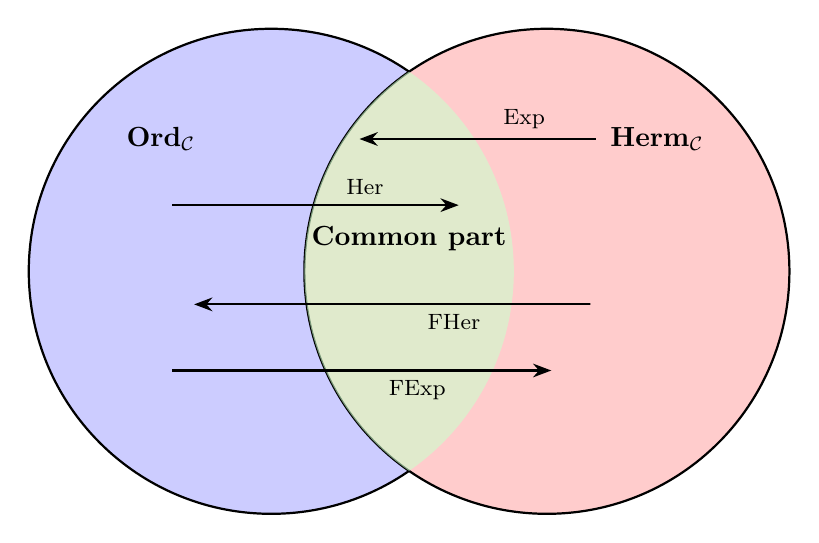
\begin{tikzpicture}[>=Stealth, scale=1.4, every node/.style={font=\small}]
  % adjustable parameters
  \def\r{2.2}   % circle radius
  \def\dx{2.5}  % distance between centers

  % left circle (Ord)
  \begin{scope}
    \clip (0,0) circle (\r);
    \fill[blue!20] (0,0) circle (\r);
  \end{scope}
  \draw[thick] (0,0) circle (\r);

  % right circle (Herm)
  \begin{scope}
    \clip (\dx,0) circle (\r);
    \fill[red!20] (\dx,0) circle (\r);
  \end{scope}
  \draw[thick] (\dx,0) circle (\r);

  % overlap (Common part) colored separately
  \begin{scope}
    \clip (0,0) circle (\r);
    \fill[green!20,opacity=0.6] (\dx,0) circle (\r);
  \end{scope}

  % labels INSIDE circles
  \node[font=\normalsize\bfseries] at (-1.0,1.2) {$\mathbf{Ord}_{\mathcal C}$};
  \node[font=\normalsize\bfseries] at (\dx+1.0,1.2) {$\mathbf{Herm}_{\mathcal C}$};
  \node[font=\normalsize\bfseries] at (0.5*\dx,0.3) {Common part};

  % Functor arrows
  % Her (Ord -> Common)
  \draw[->, thick] (-0.9,0.6) .. controls (0.5,0.6) and (1.5,0.6) .. (1.7,0.6)
    node[pos=0.5, above] {\footnotesize $\mathrm{Her}$};

  % FExp (Ord -> Herm)
  \draw[->, thick] (-0.9,-0.9) .. controls (0.5,-0.9) and (2.0,-0.9) .. (\dx4,-0.9)
    node[pos=0.55, below] {\footnotesize $\mathrm{FExp}$};

  % Exp (Herm -> Common)
  \draw[->, thick] (\dx5,1.2) .. controls (4.0,1.2) and (1.0,1.2) .. (0.8,1.2)
    node[pos=0.5, above] {\footnotesize $\mathrm{Exp}$};

  % FHer (Herm -> Ord)
  \draw[->, thick] (\dx5,-0.3) .. controls (4.0,-0.3) and (0.5,-0.3) .. (-0.7,-0.3)
    node[pos=0.55, below] {\footnotesize $\mathrm{FHer}$};

\end{tikzpicture}

\vspace{0.5em}
\footnotesize
Sequences in the common part are precisely those whose arrows are surjective ordinary maps.
\caption{Relation between $\mathbf{Ord}_{\mathcal C}$ and $\mathbf{Herm}_{\mathcal C}$. 
Object-level functors ($\mathrm{Her},\mathrm{Exp}$) land in the shared surjective core, 
while function-level functors ($\mathrm{FExp},\mathrm{FHer}$) map across the categories.}
\end{figure}
\medskip
This situation is made explicit in the following Venn diagram, which depicts how the four functors act with respect to the overlap 
between $\mathbf{Ord}_\mathcal C$ and $\mathbf{Herm}_\mathcal C$. 
For longer sequences, however, a single application of element level modification does not suffice to reach the common part. 
Rather, it becomes an important task to study how repeated iterations
\end{remark}

\begin{theorem}[Length dependence of modification functors]
Let $C$ be a category, and let
\[
O = (A_n \xrightarrow{d_n} A_{n-1} \to \cdots \to A_0) \in \mathrm{Ord}_C
\]
be a finite sequence of length $n$.

\begin{enumerate}
\item[\textup{(1)}] \textbf{Function-level modification.}
The functors
\[
\mathrm{FExp} : \mathrm{Ord}_C \to \mathrm{Herm}_C,
\quad
\mathrm{FHer} : \mathrm{Herm}_C \to \mathrm{Ord}_C
\]
act only on the level of arrows and do not modify the underlying objects.
In particular, a single application of either $\mathrm{FExp}$ or $\mathrm{FHer}$
transforms the sequence between the Hermetic and Ordinary forms
(up to the choice involved in $\mathrm{FHer}$).

Hence function-level modification is achieved in one step.

\item[\textup{(2)}] \textbf{Element-level modification.}
The functors
\[
\mathrm{Exp} : \mathrm{Herm}_C \to \mathrm{Ord}_C,
\quad
\mathrm{Her} : \mathrm{Ord}_C \to \mathrm{Herm}_C
\]
act on the level of objects and modify the underlying sets of the sequence.

In general, for a sequence of length $n$, the effect of $\mathrm{Exp}$ or $\mathrm{Her}$
does not occur simultaneously at all levels, but propagates along the sequence.
Consequently, multiple successive applications are required to fully transform
the entire sequence.

More precisely, the transformation propagates step by step along the index,
and may require up to $n-1$ iterations to affect all components.

\item[\textup{(3)}] \textbf{Asymmetry.}
There is a fundamental asymmetry between the two types of modifications:
function-level functors act locally and complete the transformation in one step,
while element-level functors act globally and require a number of steps
proportional to the length of the sequence.
\end{enumerate}
\end{theorem}

\begin{remark}
The above length dependence can be understood through the propagation
of stability along the sequence.

The terminal object $A_0$ is stable by definition. A single application
of the expansion functor propagates stability to $A_1$, and further
iterations propagate stability inductively to higher levels.

Thus, stability spreads step by step along the sequence, which explains
why element-level modifications require multiple iterations.
\end{remark}

\subsection{Induced morphisms}

The adjunctions provide units and counits
\[
\eta^{(f)}:\mathrm{Id}_{\mathbf{Ord}}\Rightarrow \mathrm{FHer}\circ\mathrm{FExp}, 
\quad \varepsilon^{(f)}:\mathrm{FExp}\circ\mathrm{FHer}\Rightarrow\mathrm{Id}_{\mathbf{Herm}},
\]
\[
\eta:\mathrm{Id}_{\mathbf{Herm}}\Rightarrow \mathrm{Her}\circ\mathrm{Exp}, 
\quad \varepsilon:\mathrm{Exp}\circ\mathrm{Her}\Rightarrow\mathrm{Id}_{\mathbf{Ord}}.
\]
By composing these units and counits we obtain natural morphisms 
from any sequence to its double modification.

\begin{proposition}
For any $O\in\mathbf{Ord}_{\mathcal C}$ and $S\in\mathbf{Herm}_{\mathcal C}$,
there exist canonical morphisms
\[
O \longrightarrow \mathrm{Exp}\circ\mathrm{FExp}(O),
\qquad
\mathrm{Her}\circ\mathrm{FHer}(S)\longrightarrow S,
\]
natural in $O$ and $S$.
\end{proposition}

\begin{proof}
The first morphism is obtained by applying the unit 
$\eta^{(f)}:O\to \mathrm{FHer}\circ\mathrm{FExp}(O)$
followed by $\mathrm{FHer}(\eta): \mathrm{FHer}\circ\mathrm{FExp}(O)\to
\mathrm{FHer}\circ\mathrm{Her}\circ\mathrm{Exp}\circ\mathrm{FExp}(O)$
and simplifying along the adjunction identities.
The second morphism is constructed dually, 
using $\eta:S\to\mathrm{Her}\circ\mathrm{Exp}(S)$
and $\varepsilon^{(f)}:\mathrm{FExp}\circ\mathrm{FHer}(S)\to S$.
Naturality follows from the functoriality of the units and counits.
\end{proof}

The functors $\mathrm{Exp}$ and $\mathrm{Her}$ act directly on the underlying 
structures that support a sequence. In other words, given an object $X$ in a 
sequence $O(X)$ or $H(X)$, the application of $\mathrm{Exp}$ or $\mathrm{Her}$ 
does not merely reindex the sequence, but transforms the ambient algebraic 
structure of $X$ itself. 

Once an object enters the \emph{common part}---that is, a position in the sequence 
where all morphisms become surjective ordinary functions---the actions of 
$\mathrm{Exp}$, $\mathrm{Her}$, $\mathrm{FExp}$, and $\mathrm{FHer}$ all become 
trivial. Formally, for any $O \in \text{Common}$ we have
\[
   \mathrm{Exp}(O) \;=\; \mathrm{Her}(O) \;=\; \mathrm{FExp}(O) \;=\; \mathrm{FHer}(O) \;=\; O.
\]

\subsection{One-step expansion and compression}

\begin{definition}[One-step expansion and compression]
We define two endofunctors as follows:
\begin{enumerate}
    \item The \emph{one-step expansion} 
    \[
    \mathbb{E} := \mathrm{Exp}\circ \mathrm{FExp} : 
    \mathbf{Ord}_{\mathcal C} \to \mathbf{Ord}_{\mathcal C}
    \]
    sends an ordinary sequence to its function-expansion 
    followed by object-expansion.
    \item The \emph{one-step compression}
    \[
    \mathbb{H} := \mathrm{Her}\circ \mathrm{FHer} : 
    \mathbf{Herm}_{\mathcal C} \to \mathbf{Herm}_{\mathcal C}
    \]
    sends a Hermetic sequence to its function-compression 
    followed by object-compression.
\end{enumerate}
\end{definition}

By the previous proposition, there exist canonical natural transformations
\[
\mathrm{Id}_{\mathbf{Ord}}\;\Rightarrow\;\mathbb{E}, 
\qquad
\mathbb{H}\;\Rightarrow\;\mathrm{Id}_{\mathbf{Herm}},
\]
expressing that one-step expansion is an enlargement 
while one-step compression is a reduction.


Let $O\in \mathbf{Ord}_\mathcal C$ be a sequence 
\[
\cdots \longrightarrow A_{n+1} \xrightarrow{d_{n+1}} A_{n} \xrightarrow{d_{n}} A_{n-1} \longrightarrow \cdots .
\]
We say that $A_k$ is a \emph{stable object} if 
\[
E(A_k) \;\cong\; A_k ,
\]
that is, $A_k$ is fixed under one-step expansion or compression. Equivalently, $A_k$ lies in the common part.


\begin{proposition}[Propagation of stability]
Let $O\in \mathbf{Ord}_\mathcal C$ be a sequence as above. 
If $A_n$ is a stable object, then in $E^k(O)$ all objects 
\[
A_{n+k},\; A_{n+k-1},\;\dots,\; A_{n}
\]
are stable for every $k\geq 0$.
\end{proposition}

\begin{proof}
Consider the local fragment 
\[
A_{m+1} \xrightarrow{d_{m+1}} A_m
\]
of the sequence. This is precisely the two-term situation analyzed earlier. 
In that case, one-step expansion turns $A_m$ into a stable object once $A_{m+1}$ has already stabilized. 

Applying this observation to the pair $(A_{n+1},A_n)$ shows that if $A_n$ is stable, then after one application of $E$, the object $A_{n+1}$ also becomes stable. Iterating the argument inductively, stability propagates along the sequence to the right: once $A_n$ is stable, so are $A_{n+1}, A_{n+2}, \dots$. 

Hence for every $k\geq 0$, the objects $A_{n+k},\dots,A_n$ are stable in $E^k(O)$. 
\end{proof}
\subsection{Some Interesting Examples of Commutative diagrams}

The relations among the four functors may be summarized 
in the following diagram. 

\begin{proposition}
Let $O\in\mathbf{Ord}_{\mathcal C}$ and $S\in\mathbf{Herm}_{\mathcal C}$. 
Assume $S\simeq \mathrm{FExp}(O)$. 
Then the two-step modifications 
$\mathbb{E}(O)=\mathrm{Exp}\circ\mathrm{FExp}(O)$ 
and $\mathbb{H}(S)=\mathrm{Her}\circ\mathrm{FHer}(S)$ 
construct a commutative diagram:
\[
\begin{tikzcd}[row sep=large, column sep=large]
O \ar[r, "\mathrm{FExp}"] \ar[d] & 
\mathrm{FExp}(O) \ar[r, "\mathrm{Exp}"] \ar[d] & 
\mathbb{E}(O) \ar[d] \\
S \ar[r, "\mathrm{FHer}"'] & 
\mathrm{FHer}(S) \ar[r, "\mathrm{Her}"'] & 
\mathbb{H}(S)
\end{tikzcd}
\]
If $\mathbb{E}(O)$ is isomorphic to $\mathbb{H}(S)$, then this commutative diagram exists up to natural isomorphism.
\end{proposition}

This commutative diagram illustrates that although object-level 
and function-level modifications act in different directions, 
their combined effects eventually converge to the common part.

From Corollary 1, the local tendency toward the common part shows that 
the essential information of the sequence after $n$ iterations of one-step expansion 
is completely determined by the positions of the stable objects already present.
Let $O_1 \in \mathbf{Ord}_\mathcal C$ be the long sequence
\[
A^0_6 \xrightarrow{d_6} A^0_5 \xrightarrow{d_5} A^0_4 \xrightarrow{d_4} A^0_3 
\xrightarrow{d_3} A^0_2 \xrightarrow{d_2} A^0_1 \xrightarrow{d_1} 0,
\]
where $d_5$ is assumed to be surjective. Then we obtain the following commutative diagram:
\[
\begin{tikzcd}[row sep=2.5em, column sep=3.5em]
A^0_6 \arrow[r]\arrow[d,"d_6"'] 
  & A^1_6 \arrow[dl,"e_6"']  
  & {} & {} \\
A^0_5 \arrow[d,"d_5"'] 
  & {} & {} & {} \\
A^0_4 \arrow[r]\arrow[d,"d_4"'] 
  & A^1_4 \arrow[r]\arrow[d,"e_4"']  
  & A^2_4 \arrow[r]\arrow[d,"f_4"']
  & A^3_4  \arrow[dl,"g_4"'] \\
A^0_3 \arrow[r]\arrow[d,"d_3"'] 
  & A^1_3 \arrow[r]\arrow[d,"e_3"'] 
  & A^2_3 \arrow[dl,"f_3"']
  & {} \\
A^0_2 \arrow[r]\arrow[d,"d_2"'] 
  & A^1_2 \arrow[dl,"e_2"'] 
  & {} & {} \\
A^0_1 \arrow[d,"d_1"'] 
  & {} & {} & {} \\
0 & {} & {} & {}
\end{tikzcd}
\]


Here, vertical maps in the second and third columns are labeled $e_4, e_3, e_2$ and $f_4$ respectively, 
while the diagonal maps are $e_6$ (from $A^1_6$ to $A^0_5$) and $g_4,f_3,e_2$ (from $A^3_4$ to $A^0_1$).
The stable objects in this diagram are highlighted in red:
\[
\boxed{A^0_1, \; A^1_2, \; A^2_3, \; A^3_4, \; A^1_6, \; A^0_5}.
\]
All maps between these stable objects are surjective.



\paragraph{Horizontal and vertical short sequences.}
Starting from an ordinary object $(C_1\in \mathbf{Ord}_\mathcal C: A \longrightarrow B)$, we obtain the horizontal short sequence
\[
   O(C_1) \;\longrightarrow\; H(C_1) \;\longrightarrow\; O(D_1),
\]
whose terminal entry $O(D_1)$ belongs to the common part.  
Dually, beginning at $H(C_1)$ we obtain the vertical short sequence
\[
   H(C_1) \;\longrightarrow\; O(C_2) \;\longrightarrow\; H(C_2'),
\]
whose terminal $H(C_2')$ also lies in the common part.

\begin{theorem}[Alternating diagram]
By splicing together the horizontal and vertical short sequences, one obtains the 
following alternating diagram:

\begin{figure}[h]
\centering
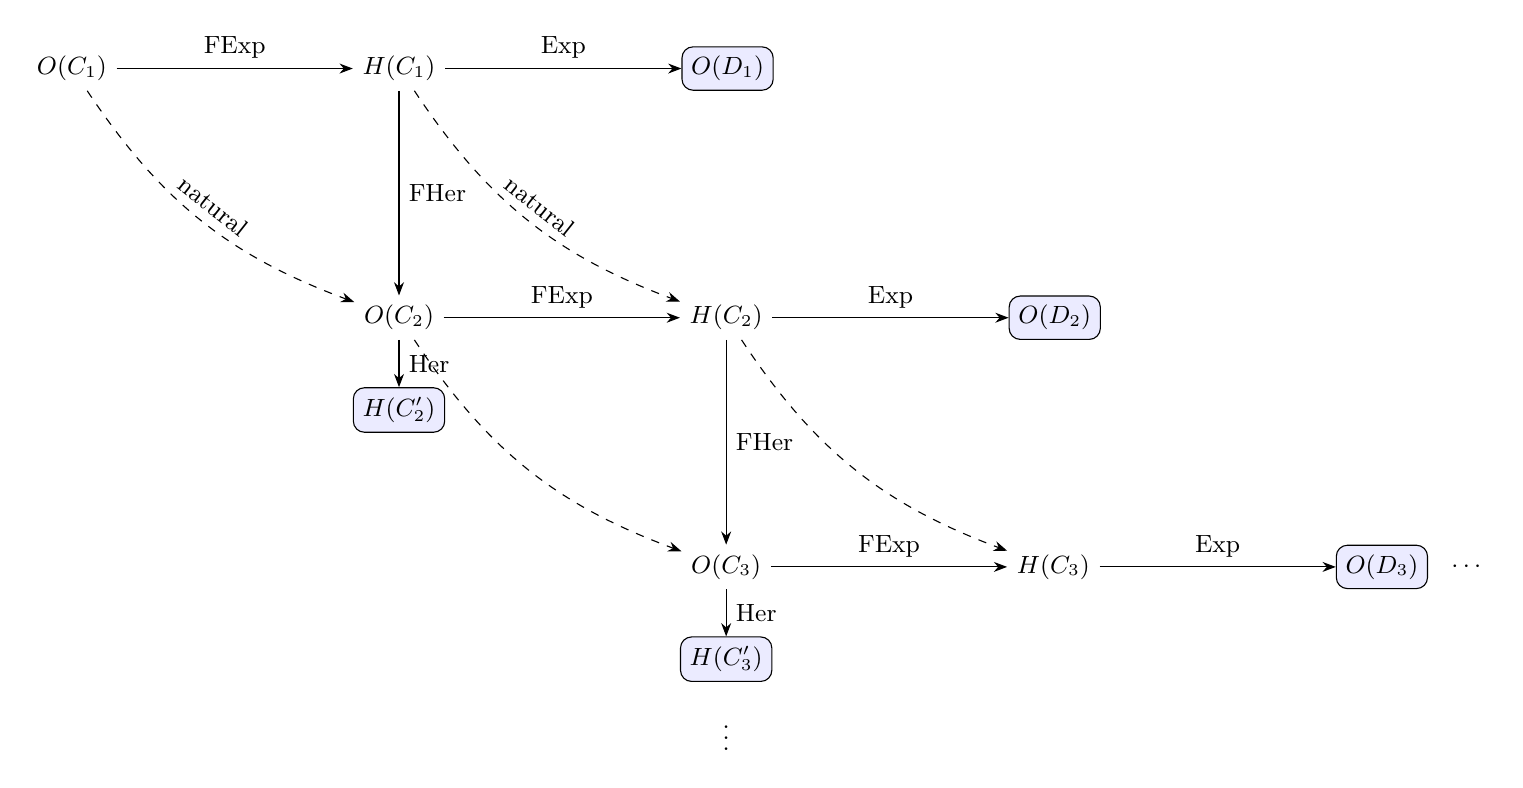
\begin{tikzpicture}[>=Stealth, font=\small, node distance=2.6cm and 3.0cm]
  % Row 1
  \node (O1) {$O(C_1)$};
  \node (H1) [right=of O1] {$H(C_1)$};
  \node (D1) [right=of H1, draw,rounded corners,fill=blue!8] {$O(D_1)$};

  % Row 2: O2 directly below H1; H2 to the right of O2; D2 to the right of H2
  \node (O2) [below=of H1] {$O(C_2)$};        % directly under H1
  \node (H2) [right=of O2] {$H(C_2)$};
  \node (D2) [right=of H2, draw,rounded corners,fill=blue!8] {$O(D_2)$};

  % Column terminal under O2
  \node (H2p) [below=6mm of O2, draw,rounded corners,fill=blue!8] {$H(C_2')$};

  % Row 3: O3 below H2; H3 right of O3; D3 right of H3
  \node (O3) [below=of H2] {$O(C_3)$};
  \node (H3) [right=of O3] {$H(C_3)$};
  \node (D3) [right=of H3, draw,rounded corners,fill=blue!8] {$O(D_3)$};

  % Column terminal under O3
  \node (H3p) [below=6mm of O3, draw,rounded corners,fill=blue!8] {$H(C_3')$};

  % --- Horizontal arrows (solid) ---
  \draw[->] (O1) -- node[above]{\small FExp} (H1);
  \draw[->] (H1) -- node[above]{\small Exp} (D1);

  \draw[->] (O2) -- node[above]{\small FExp} (H2);
  \draw[->] (H2) -- node[above]{\small Exp} (D2);

  \draw[->] (O3) -- node[above]{\small FExp} (H3);
  \draw[->] (H3) -- node[above]{\small Exp} (D3);

  % --- Vertical / weaving arrows (solid) ---
  \draw[->] (H1) -- node[right]{\small FHer} (O2);
  \draw[->] (O2) -- node[right]{\small Her} (H2p);

  \draw[->] (H2) -- node[right]{\small FHer} (O3);
  \draw[->] (O3) -- node[right]{\small Her} (H3p);

  % --- Diagonal natural chains (dashed) connecting same-type nodes ---
  \draw[dashed,->] (O1) to[bend right=18] node[sloped, above]{\small natural} (O2);
  \draw[dashed,->] (O2) to[bend right=18] (O3);

  \draw[dashed,->] (H1) to[bend right=18] node[sloped, above]{\small natural} (H2);
  \draw[dashed,->] (H2) to[bend right=18] (H3);

  % continuation dots (optional)
  \node at ($(D3)+(1.1,0)$) {$\cdots$};
  \node at ($(H3p)+(0,-0.9)$) {$\vdots$};
\end{tikzpicture}
\caption{Alternating $O\!-\!H\!-\!O\!-\!H$ grid. Horizontal and vertical arrows are solid; diagonal same-type natural maps are dashed.}
\label{fig:OHOH-grid}
\end{figure}

Each horizontal row and vertical column terminates in the common part, highlighted 
as blue nodes in the diagram.
\end{theorem}

If we disregard the terminal entries lying in the common part, the diagram reduces 
to an infinite alternating chain of the form
\[
   O(C_1) \;\to\; H(C_1) \;\to\; O(C_2) \;\to\; H(C_2) \;\to\; O(C_3) \;\to\; \cdots,
\]
which we call the \emph{$OHOH$-sequence}. Along this sequence, there exist two 
parallel families of natural transformations: one running along the $O$-objects, 
and the other along the $H$-objects, both induced by the units and counits of the 
adjunctions $\mathrm{FExp}\dashv\mathrm{FHer}$ and $\mathrm{Exp}\dashv\mathrm{Her}$.

Among this \emph{$OHOH$-sequence}, there exists a commutataive diagram of $O(C_i)$ :
\[
\begin{tikzcd}[row sep=3em, column sep=4em]
A_1 \arrow[r,"\cong"] \arrow[d] & A_2 \arrow[r,"\cong"] \arrow[d] & A_3 \arrow[r,"\cong"] \arrow[d] & \cdots \\
B_1 \arrow[r,"\cong"]           & B_2 \arrow[r,"\cong"]           & B_3 \arrow[r,"\cong"]           & \cdots
\end{tikzcd}
\]

\chapter{Hermetic Sequence in Graph Theory}

This chapter develops a dynamical and operator-algebraic framework
associated with Hermetic sequences.

Starting from the combinatorial structure of a sequence,
we construct an associated directed graph and its path space.
This naturally leads to a shift dynamical system,
together with a canonical involution reflecting reversal symmetry.

We then show that these structures generate natural algebraic objects,
including a graph $C^*$-algebra and a dihedral group action.

\section{Graph Structure of Hermetic Sequences}

We begin by encoding Hermetic sequences into directed graphs.
This allows us to translate the combinatorial structure
into a geometric and visual framework.

The resulting graph is naturally layered,
reflecting the level structure of the sequence,
and serves as the foundation for all subsequent constructions.

\begin{proposition}
The category $\mathrm{Seq}(\mathcal C)$ embeds into the category
$\mathrm{Grph}$ of directed graphs.
\end{proposition}

\begin{proof}
Given a sequence
\[
A_n \xrightarrow{F_n} A_{n-1} \to \cdots \to A_0
\]
we construct a directed graph whose vertices are the elements
of the sets $A_i$ and whose edges are given by the arrows
\[
a \to F_i(a).
\]
This construction is functorial with respect to sequence morphisms,
hence defines an embedding
\[
\mathrm{Seq}(\mathcal C) \hookrightarrow \mathrm{Grph}.
\]
\end{proof}

\begin{definition}[Sequence graph]
Let
\[
A_n \to A_{n-1} \to \cdots \to A_0
\]
be a sequence.

The sequence graph is the directed graph whose vertices
are finite sequences
\[
(a_k,\dots,a_0)
\]
compatible with the arrows of the sequence, and whose edges
are given by truncation of the last element.
\end{definition}

\begin{definition}[sequence path]
Let $(A_n,F_n)$ be a sequence.
A finite path is a sequence of arrows
\[
f_{i_1},f_{i_2},\dots,f_{i_k}
\]
such that
\[
\operatorname{cod}(f_{i_j})=\operatorname{dom}(f_{i_{j+1}})
\]
for all $j$.
\end{definition}

While the graph captures the local structure of the sequence,
its global behavior is more naturally described in terms of paths.

We therefore pass from the graph itself
to the associated path space,
which encodes all possible evolutions within the structure.

\begin{definition}[Path space of a sequence]
Let $G$ be a directed graph.

The path space of $G$ is the set of all directed paths
(finite or infinite) in $G$.

Particularly, for a sequence:
\[
A_n \to A_{n-1} \to \cdots \to A_0
\],

the path space consists of all sequences
\[
(a_k,a_{k-1},\dots,a_0)
\]
such that
\[
a_i \mapsto a_{i-1}.
\]
\end{definition}

\begin{proposition}[Bounded path length]
Let
\[
A_n \to A_{n-1} \to \cdots \to A_0
\]
be a finite sequence.

Then every directed path in the associated graph
has length at most $n$.

\end{proposition}

A hermetic sequence graph differs from a finite Bratteli diagram in that the covering condition is imposed
only on the lower level. Every vertex in $A_{n-1}$ must receive at least one edge from the level above, 
while vertices in $A_n$ are not required to emit edges. 

\begin{proposition}
A hermetic sequence graph has following 
properties:

1.Every sequence graph is a layered directed graph whose
edges only connect adjacent layers.

2.In a Hermetic sequence, every vertex admits
a path descending to level $0$.

3.Every infinite Hermetic sequence admits at least one infinite path.

4.Branching in a Hermetic sequence occurs exactly
at vertices with multiple outgoing edges.

5.Vertices of the sequence graph correspond to
finite directed paths in the original sequence.
\end{proposition}

\begin{proposition}[Backward traceability]
Let $G$ be the directed graph associated with a Hermetic sequence.
Then every vertex of $G$ has at least one predecessor; that is,
for every vertex $v$ there exists a vertex $u$ such that
\[
u \to v
\]
is an edge of $G$.

Consequently, every vertex belongs to at least one backward path
reaching a higher level of the sequence.
\end{proposition}

We now introduce a dynamical viewpoint on sequences by considering
their associated path spaces.  

It is standard in the study of directed graphs
to pass from the graph itself to its associated path space,
which captures the global combinatorial and dynamical behavior.

Following this perspective,
we consider the space of infinite paths in the graph.

Moreover, unlike the Hermetic-specific construction discussed earlier, 
the following definitions apply to arbitrary sequences in the category $\mathrm{Seq}$.

\begin{definition}[Infinite sequence path]
Let $(A_n,F_n) \in \mathrm{Seq}$ be a sequence
\[
\cdots \xrightarrow{F_{n+1}} A_n \xrightarrow{F_n} A_{n-1}
\xrightarrow{F_{n-1}} \cdots \xrightarrow{F_1} A_0 .
\]

An \emph{infinite sequence path} is a sequence of elements
\[
x = (\ldots, a_2, a_1, a_0)
\]
such that for every $n \ge 1$ the elements satisfy the compatibility
condition
\[
a_n \xrightarrow{F_n} a_{n-1}.
\]

The set of all infinite sequence paths will be denoted by
\[
X(A_\bullet,F_\bullet),
\]
and called the \emph{path space} of the sequence.
\end{definition}

\begin{corollary}[Well-definedness in the Hermetic case]
Let $(A_n,F_n)$ be a Hermetic sequence.
Then the shift map
\[
\sigma : X(A_\bullet,F_\bullet) \to X(A_\bullet,F_\bullet)
\]
is well-defined.

\emph{Proof.}
Let $x=(\ldots,a_2,a_1,a_0)$ be a path.
By definition we have
\[
a_n \xrightarrow{F_n} a_{n-1}
\]
for all $n$.
Removing the last element $a_0$ produces the sequence
$(\ldots,a_2,a_1)$, which still satisfies the same compatibility
conditions.
Hence the resulting sequence remains a valid path.
\hfill $\square$
\end{corollary}

\section{Graph-theoretic Interpretation of the Modification Functors}

In the previous sections, we introduced four modification functors:
\[
\mathrm{Exp}, \quad \mathrm{Her}, \quad \mathrm{FExp}, \quad \mathrm{FHer}.
\]

The graph structures introduced above are not arbitrary:
they arise naturally from the modification functors defined in Chapter 3.
We now make this correspondence explicit. We now reinterpret these functors in the language of graph theory.

We show that each functor corresponds naturally to a local transformation
of the directed graph associated with a Hermetic sequence.
More precisely, they correspond to four fundamental graph operations:
vertex splitting, pruning, edge duplication, and edge selection.

\medskip

\textbf{(1) Expansion as vertex splitting.}

The functor $\mathrm{Exp}$ acts on objects by introducing labels,
replacing each element with a family of labeled copies.

In graph-theoretic terms, this corresponds to a vertex-splitting operation.
Each vertex $a \in A_n$ is replaced by vertices $(a,\alpha)$,
where $\alpha$ ranges over the outgoing branches of $a$.
Edges are then reassigned so that each new vertex has exactly one outgoing edge.

Thus, a multi-valued correspondence is transformed into a deterministic graph.

\medskip

\textbf{(2) Hermetization as pruning.}

The functor $\mathrm{Her}$ acts by restricting to the image of the previous level.

In graph-theoretic terms, this corresponds to a pruning operation.
Vertices that do not lie in the image of any incoming edge are removed,
resulting in a subgraph in which every vertex admits at least one predecessor.

This enforces the traceability condition at the graph level.

\medskip

\textbf{(3) Function expansion as edge duplication.}

The functor $\mathrm{FExp}$ replaces a function by a singleton family.

In graph-theoretic terms, each edge is lifted to a family-valued edge.
This may be interpreted as a formal duplication or labeling of edges,
embedding single-valued edge structures into a family-valued framework.

\medskip

\textbf{(4) Function Hermetization as edge selection.}

The functor $\mathrm{FHer}$ selects a single function from a family.

In graph-theoretic terms, this corresponds to selecting one outgoing edge at each vertex,
thereby producing a deterministic subgraph.
This selection defines a path system within the original graph.

\medskip

In summary, the four modification functors correspond to four fundamental graph operations:
\[
\text{vertex splitting}, \quad \text{pruning}, \quad \text{edge duplication}, \quad \text{edge selection}.
\]

This correspondence provides a bridge between the categorical structure of Hermetic sequences
and the combinatorial structure of directed graphs,
which will be further exploited in the study of dynamical systems and operator algebras.


\section{Shift Dynamics}
The path space admits a natural shift operation,
which advances along paths by one step.
This endows the space with a dynamical system structure.

In the Hermetic setting, this shift is well-defined
due to the backward traceability condition,
which ensures the existence of compatible extensions.
\begin{definition}[Shift map]
Let $X(A_\bullet,F_\bullet)$ be the path space of a sequence
$(A_n,F_n) \in \mathrm{Seq}$.

The \emph{shift map}
\[
\sigma : X(A_\bullet,F_\bullet) \longrightarrow X(A_\bullet,F_\bullet)
\]
is defined by
\[
\sigma(\ldots,a_2,a_1,a_0) = (\ldots,a_2,a_1).
\]

That is, the shift map removes the lowest-level element of the path.
\end{definition}

\begin{definition}[Sequence dynamical system]
Let $(A_n,F_n)\in \mathrm{Seq}$ and let
$X(A_\bullet,F_\bullet)$ denote its path space.
The pair
\[
\bigl(X(A_\bullet,F_\bullet),\sigma\bigr)
\]
is called the \emph{sequence dynamical system} associated with the
sequence.
\end{definition}

The shift map on the path space
induces a natural representation on the Hilbert space $\ell^2(X)$.

This connects the dynamical system
to operator-theoretic structures.

\begin{definition}[Tail equivalence]
Let $(A_n,F_n) \in \mathrm{Seq}$ and let
\[
X(A_\bullet,F_\bullet)
\]
be its path space.

Two paths
\[
x=(\ldots,a_2,a_1,a_0),
\qquad
y=(\ldots,b_2,b_1,b_0)
\]
are said to be \emph{tail equivalent} if there exists
$N \ge 0$ such that
\[
a_n = b_n
\]
for all $n \ge N$.

This relation will be denoted by
\[
x \sim_{\mathrm{tail}} y .
\]
\end{definition}

The tail equivalence relation on the path space admits
a natural groupoid structure.

Such equivalence relations are well known
to give rise to groupoid structures
in the study of AF $C^*$-algebras and related dynamical systems.

Motivated by this framework,
we equip the tail equivalence relation with a natural groupoid structure.

\begin{definition}[Tail groupoid]
Let $(A_n,F_n)\in \mathrm{Seq}$ and let
$X(A_\bullet,F_\bullet)$ denote its path space.

The \emph{tail groupoid} associated with the sequence
is the set
\[
G_{\mathrm{tail}}
=
\{(x,k,y) \mid x,y\in X(A_\bullet,F_\bullet),\;
k\in \mathbb{Z},\;
\sigma^k(x)=y \}.
\]

The groupoid operations are defined as follows.

\begin{itemize}
\item
Composition:
\[
(x,k,y)\cdot(y,l,z)=(x,k+l,z)
\]

\item
Inverse:
\[
(x,k,y)^{-1}=(y,-k,x)
\]

\item
Units:
\[
(x,0,x)
\]
for all $x\in X(A_\bullet,F_\bullet)$.
\end{itemize}
\end{definition}

This groupoid encodes the shift dynamics on the path space,
and may be viewed as a dynamical groupoid associated with
the sequence.

We now introduce a transformation which interchanges
elements and morphisms in a Hermetic sequence.
This construction is specific to Hermetic sequences,
since the Hermetic condition guarantees that every
element arises as the image of some morphism.

\begin{definition}[Sequence reversal]
Let
\[
(A_n,F_n)
\]
be a Hermetic sequence. The \emph{sequence reversal}
is the transformation
\[
I : \mathrm{Herm} \longrightarrow \mathrm{Herm}
\]
defined by interchanging elements and morphisms along
the sequence.

More precisely, an element $a_n \in A_n$ determines
a morphism in the reversed sequence through its
incoming map
\[
F_{n+1}(\cdot)=a_n,
\]
while each morphism
\[
F_n : A_n \to A_{n-1}
\]
is regarded as an element of the reversed sequence.

Thus the reversed sequence is obtained by replacing
the alternating structure
\[
\cdots \to A_{n+1} \xrightarrow{F_{n+1}} A_n
\xrightarrow{F_n} A_{n-1} \to \cdots
\]
with the sequence in which morphisms play the role
of elements and elements play the role of morphisms.
\[\cdots \to F_{n+1} \xrightarrow{A_n} F_n \to \cdots\]
\end{definition}

The Hermetic condition is stable under the reversal
transformation. This ensures that the transformation
acts within the category $\mathrm{Herm}$.

\begin{proposition}
The reversal transformation
\[
I : \mathrm{Herm} \to \mathrm{Herm}
\]
is well-defined.
\end{proposition}

\begin{proof}
Let $(A_n,F_n)$ be a Hermetic sequence.
By definition, the Hermetic condition states that every
element $a_n\in A_n$ admits at least one incoming morphism,
that is, there exists $x\in A_{n+1}$ such that
\[
F_{n+1}(x)=a_n .
\]

The transformation $I$ interchanges elements and morphisms
without introducing new vertices or edges. Each morphism
$F_n$ is regarded as an element in the reversed sequence,
while each element $a_n$ determines a morphism through its
incoming relation.

Since every element has at least one incoming morphism,
every element in the reversed sequence likewise admits an
incoming relation. Hence the Hermetic condition is preserved
under the transformation.

Therefore the reversed sequence is again Hermetic, and the
map
\[
I : \mathrm{Herm} \to \mathrm{Herm}
\]
is well-defined.
\end{proof}

\begin{remark}
The transformation $I$ is well-defined only for
Hermetic sequences. Indeed, the Hermetic condition
ensures that every element $a_n$ admits at least one
incoming morphism
\[
F_{n+1}(x)=a_n.
\]
This guarantees that elements can be interpreted as
arrows in the reversed sequence.
\end{remark}


Here we give an example: 

Consider the fragment
\[
a_1 \xrightarrow{f_1} b_1 \xrightarrow{g_1} c_1,
\qquad
a_2 \xrightarrow{f_2} b_1 \xrightarrow{g_2} c_2 .
\]

After applying the reversal transformation, the
morphisms become elements and the intermediate
element becomes a morphism. The resulting structure
is
\[
f_1 \xrightarrow{b_1} g_1,
\qquad
f_2 \xrightarrow{b_1} g_2 .
\]

This construction is possible because the underlying
relations between domain and codomain are many-to-many,
allowing the interchange of elements and morphisms.



\begin{theorem}
Let $(A_n,F_n)$ be an infinite Hermetic sequence.
Then the reversal transformation satisfies
\[
I^2 = \mathrm{id}.
\]
\end{theorem}

\begin{proof}
Applying $I$ once exchanges elements with morphisms.
Applying $I$ again performs the same interchange
once more, thereby restoring the original structure.
The assumption that the sequence is infinite ensures
that no boundary effects occur at the ends of the
sequence. Hence the original sequence is recovered,
and therefore
\[
I^2=\mathrm{id}.
\]
\end{proof}

\begin{proposition}
Let $(A_n,F_n)$ be an infinite Hermetic sequence and
let $X$ denote its path space. Let
\[
\sigma : X \to X
\]
be the shift map and
\[
I : X \to X
\]
the reversal transformation. Then
\[
I\circ\sigma = \sigma^{-1}\circ I .
\]
\end{proposition}

\begin{proof}
Let
\[
x=(\ldots,a_2,a_1,a_0)
\]
be a path in $X$.

Applying the shift first gives
\[
\sigma(x)=(\ldots,a_2,a_1).
\]

The reversal transformation exchanges elements with the
morphisms determined by their incoming relations.
Hence
\[
I(\sigma(x))
\]
produces the reversed sequence associated with the
truncated path.

On the other hand, applying the reversal first yields
a path whose elements correspond to the morphisms of
the original sequence. Shifting this reversed path
in the opposite direction restores the same alignment
of elements and morphisms.

Therefore
\[
I(\sigma(x))=\sigma^{-1}(I(x)).
\]

Thus
\[
I\circ\sigma = \sigma^{-1}\circ I .
\]
\end{proof}

\section{Algebra Generated from Hermetic Sequences}
Let $(A_n,F_n)$ be a Hermetic sequence and let
$G$ denote the directed graph associated with it.
The vertices of $G$ are the elements of the sets $A_n$
and the edges correspond to the morphisms in $F_n$.

By the Hermetic condition every vertex has at least
one incoming edge, while the number of outgoing edges
may be zero or greater.

We now associate a $C^*$-algebra to this graph.

\begin{definition}[Hermetic graph algebra]
Let $G=(V,E)$ be the graph associated with a Hermetic
sequence. The \emph{Hermetic graph $C^*$-algebra}
$C^*(G)$ is the universal $C^*$-algebra generated by

\[
\{p_v : v\in V\}, \qquad \{s_e : e\in E\}
\]

subject to the relations

\begin{enumerate}
\item $p_v$ are mutually orthogonal projections,

\[
p_v p_w = 0 \quad (v\neq w)
\]

\item $s_e$ are partial isometries,

\[
s_e^* s_e = p_{r(e)}
\]

\item

\[
s_e s_e^* \le p_{s(e)}
\]

\item for every vertex $v$ with finitely many outgoing edges,

\[
p_v=\sum_{s(e)=v} s_e s_e^* .
\]

\end{enumerate}

The algebra satisfying these relations is denoted
\[
C^*(G).
\]
\end{definition}

\begin{proposition}
Let $X$ be the infinite path space of the Hermetic
sequence. The shift map

\[
\sigma:X\to X
\]

induces a representation of the generators of $C^*(G)$
on $\ell^2(X)$.
\end{proposition}

Let $(A_n,F_n)$ be a Hermetic sequence and let
$G=(V,E)$ be the associated directed graph, where

\[
V=\bigcup_n A_n
\]

and edges correspond to morphisms in the sets $F_n$.

Therefore, in addition to the graph algebra,
we introduce a $*$-algebra structure
directly on the sequence itself.

This algebra reflects the intrinsic symmetries
of Hermetic sequences.

Through observation, by the Hermetic condition, every vertex has at least
one incoming edge, while the number of outgoing edges
may be zero or greater.

We now construct an algebraic structure induced by
the reversal transformation.

Let $\mathrm{Herm}$ denote the class of Hermetic
sequences and let

\[
I:\mathrm{Herm}\to\mathrm{Herm}
\]

be the reversal transformation exchanging elements
and morphisms.

For an infinite Hermetic sequence one has

\[
I^2=\mathrm{id}.
\]

\begin{definition}[Sequence $*$-algebra]
Let $\mathcal{A}$ be the algebra generated by the
formal symbols corresponding to elements and
morphisms of a Hermetic sequence.

The involution

\[
*: \mathcal{A}\to\mathcal{A}
\]

is defined by

\[
x^* = I(x).
\]

The pair $(\mathcal{A},*)$ is called the
\emph{sequence $*$-algebra} associated with the
Hermetic sequence.
\end{definition}

\begin{proposition}
For an infinite Hermetic sequence the involution
satisfies

\[
(x^*)^* = x .
\]
\end{proposition}

\begin{proof}
This follows from the identity
\[
I^2=\mathrm{id}.
\]
\end{proof}

Let $X$ be the infinite path space of a Hermetic
sequence. The shift map

\[
\sigma : X \to X
\]

and the reversal transformation

\[
I : X \to X
\]

satisfy

\[
I^2=\mathrm{id}, \qquad
I\sigma I=\sigma^{-1}.
\]

\begin{definition}
The group generated by $\sigma$ and $I$

\[
\langle \sigma , I \rangle
\]

is called the \emph{dihedral symmetry group}
of the Hermetic system.
\end{definition}

\begin{proposition}
The group generated by $\sigma$ and $I$ is
isomorphic to the infinite dihedral group

\[
D_\infty .
\]
\end{proposition}

\begin{proof}
The generators satisfy

\[
I^2=1, \qquad I\sigma I=\sigma^{-1},
\]

which is the standard presentation of the
infinite dihedral group.
\end{proof}

In the three definitions before, we introduced the path space
of a Hermetic sequence together with the shift dynamics
and the reversal transformation.

These transformations naturally generate several
algebraic structures associated with the Hermetic system.
They arise from three fundamental operations:

\begin{itemize}
\item the shift map $\sigma$ on the path space,
\item the reversal transformation $I$ exchanging elements
and morphisms,
\item the relation between them,
\[
I\sigma I = \sigma^{-1}.
\]
\end{itemize}

Each of these operations gives rise to a corresponding
algebraic structure. The following table summarizes
this correspondence.

\begin{center}
\begin{tabular}{c|c}
Transformation / Relation & Associated Algebra \\ \hline

Shift $\sigma$ & Hermetic graph $C^*$-algebra $C^*(G)$ \\

Reversal $I$ & Sequence $*$-algebra $(\mathcal A,*)$ \\

Relation $I\sigma I=\sigma^{-1}$ & Infinite dihedral group $D_\infty$

\end{tabular}
\end{center}

These three structures reflect different aspects of the
Hermetic system. The graph $C^*$-algebra arises from the
combinatorial structure of the associated directed graph,
the sequence $*$-algebra is induced by the symmetry
between elements and morphisms, and the dihedral group
captures the interaction between the shift dynamics and
the reversal transformation.

In the following sections we study these algebras and
their relations.

Let $\sigma$ be the shift transformation on the infinite
path space $X$ of a Hermetic sequence.

The group generated by $\sigma$ is

\[
\langle \sigma \rangle
=
\{\sigma^n : n\in\mathbb Z\}.
\]

This group is called the shift group.

\begin{proposition}
The group generated by $\sigma$ is an infinite cyclic group.
\end{proposition}

\begin{proof}
For an infinite path the shift map never returns a path
to itself after finitely many iterations. Hence
$\sigma^n\neq id$ for every nonzero integer $n$.
Therefore the group generated by $\sigma$ is infinite
cyclic.
\end{proof}

Consequently
\[
\langle\sigma\rangle \cong \mathbb Z .
\]

Let $I$ be the reversal transformation.
The set
\[
\{id,I\}
\]
forms a group of order two.
Similarly
\[
\{id,I\} \cong \mathbb{Z}_2
\]

\begin{proposition}
Let $\sigma$ be the shift map and $I$ the reversal
transformation. Then

\[
I^2 = id,
\qquad
I\sigma I = \sigma^{-1}.
\]

Hence the group generated by $\sigma$ and $I$
is isomorphic to the infinite dihedral group

\[
D_\infty \cong
\mathbb Z \rtimes \mathbb Z_2 .
\]
\end{proposition}

The dihedral symmetry generated by the shift
and the reversal transformation acts naturally
on the Hermetic graph algebra.

This allows us to form the crossed product
algebra
\[
C^*(G)\rtimes D_\infty .
\]

\begin{lemma}
The reversal transformation $I$ of a Hermetic sequence
induces a $*$-automorphism of the Hermetic graph
$C^*$-algebra $C^*(G)$.
\end{lemma}

\begin{proof}
The transformation $I$ exchanges elements and morphisms
while preserving the incidence relations of the associated
graph. Hence it sends generators of $C^*(G)$ to generators
and preserves the defining relations of the algebra.
Therefore $I$ extends to a $*$-automorphism of $C^*(G)$.
\end{proof}

$\sigma$ denotes the shift transformation and
$I$ denotes the reversal transformation.
The induced automorphisms on $C^*(G)$ satisfy

\[
I^2 = id, \qquad I\sigma I = \sigma^{-1}.
\]

Hence they generate an \emph{action} of the infinite
dihedral group
\[
D_\infty
\]
on the algebra $C^*(G)$.

\begin{definition}
Since the infinite dihedral group $D_\infty$
acts on the Hermetic graph algebra $C^*(G)$
by $*$-automorphisms, we define the
\emph{Hermetic crossed product algebra}

\[
C^*(G)\rtimes D_\infty .
\]
\end{definition}

thus incorporates both the shift dynamics and
the reversal symmetry of the Hermetic system
into a single algebraic structure.

In summary, Hermetic sequences give rise to a rich hierarchy of structures:
from graphs and path spaces to dynamical systems and operator algebras.

This unified framework reveals a deep connection
between combinatorics, dynamics, and algebra.

\bibliographystyle{plain}
\bibliography{refs}

\begin{thebibliography}{9}

\bibitem{maclane}
Saunders Mac Lane,
\textit{Categories for the Working Mathematician},
Springer, 1998.

\bibitem{raeburn}
Iain Raeburn,
\textit{Graph Algebras},
CBMS Regional Conference Series in Mathematics, vol. 103,
American Mathematical Society, 2005.

\bibitem{bratteli}
Ola Bratteli,
Inductive limits of finite dimensional $C^*$-algebras,
\textit{Transactions of the American Mathematical Society},
\textbf{171} (1972), 195-234.

\bibitem{renault}
Jean Renault,
\textit{A Groupoid Approach to $C^*$-Algebras},
Lecture Notes in Mathematics, vol. 793,
Springer, 1980.

\bibitem{lindmarcus}
Douglas Lind and Brian Marcus,
\textit{An Introduction to Symbolic Dynamics and Coding},
Cambridge University Press, 1995.

\bibitem{murphy}
Gerard J. Murphy,
\textit{$C^*$-Algebras and Operator Theory},
Academic Press, 1990.

\end{thebibliography}

\end{document}